% Copyright 2004 by Till Tantau <tantau@users.sourceforge.net>.
%
% In principle, this file can be redistributed and/or modified under
% the terms of the GNU Public License, version 2.
%
% However, this file is supposed to be a template to be modified
% for your own needs. For this reason, if you use this file as a
% template and not specifically distribute it as part of a another
% package/program, I grant the extra permission to freely copy and
% modify this file as you see fit and even to delete this copyright
% notice. 


\documentclass{beamer}
\usepackage[utf8]{inputenc}


%%para criar handouts
%\documentclass[handout]{beamer}
%\usepackage[utf8]{inputenc}
%\usepackage{pgfpages}
%\usepackage{handoutWithNotes}
%\pgfpagesuselayout{4 on 1 with notes}[a4paper,border shrink=5mm]



%%%%%%%%%%%%%%%%    PREAMBLE in presentation.preamble.tex     %%%%%%%%%%%%%%%%%



\usepackage{multirow}
\usepackage{epstopdf}
\usepackage{float}
\usepackage{graphicx}
\usepackage{caption}
\usepackage{subcaption}
\usepackage{epstopdf}
\usepackage{hyperref}
\usepackage{acronym}


\setbeamertemplate{caption}[numbered]

%\usepackage{notoccite}
%\usepackage{cite}
%\\usepackage{biblatex}

\newcommand\Fontvi{\fontsize{10}{6}\selectfont}
\newcommand\Fontci{\fontsize{8}{7.2}\selectfont}
% There are many different themes available for Beamer. A comprehensive
% list with examples is given here:
% http://deic.uab.es/~iblanes/beamer_gallery/index_by_theme.html
% You can uncomment the themes below if you would like to use a different
% one:
%\usetheme{AnnArbor}
%\usetheme{Antibes}
%\usetheme{Bergen}
%\usetheme{Berkeley}
%\usetheme{Berlin}
%\usetheme{Boadilla}
%\usetheme{boxes}
%\usetheme{CambridgeUS}
%\usetheme{Copenhagen}
%\usetheme{Darmstadt}
%\usetheme{default}
%\usetheme{Frankfurt}
%\usetheme{Goettingen}
%\usetheme{Hannover}
%\usetheme{Ilmenau}
%\usetheme{JuanLesPins}
%\usetheme{Luebeck}
\usetheme{Madrid}
%\usetheme{Malmoe}
%\usetheme{Marburg}
%\usetheme{Montpellier}
%\usetheme{PaloAlto}
%\usetheme{Pittsburgh}
%\usetheme{Rochester}
%\usetheme{Singapore}
%\usetheme{Szeged}
%\usetheme{Warsaw}


\usepackage[absolute,overlay]{textpos}

\definecolor{FEUP_color}{RGB}{140,45,25}

\setbeamercolor{structure}{fg=FEUP_color}

\usepackage{booktabs}
\usepackage{multirow}

\usepackage{mdframed}



%%%%%%%%%%%%%%%%           BEGGINNING OF PRESENTATION         %%%%%%%%%%%%%%%%%

\title[]{Railway Smart Meters}

% A subtitle is optional and this may be deleted
\subtitle{Thesis Research Plan}

\author[0]{  \textbf{Vítor A. Morais}  \\ 
	        \small{Supervisor: António P. Martins (UPorto)} \\
        	\small{Co-supervisor: João L. Afonso (UMinho)} 
        }
% - Give the names in the same order as the appear in the paper.
% - Use the \inst{?} command only if the authors have different
%   affiliation.

\institute[] % (optional, but mostly needed)
{
  %\inst{1}%
  Doctoral Program in Electrical and Computer Engineering\\
  Department of Electrical and Computer Engineering\\
  Engineering Faculty --- University of Porto
  \and
  \inst{ }%
   }
% - Use the \inst command only if there are several affiliations.
% - Keep it simple, no one is interested in your street address.

\date{November 23, 2017}%\today}
% - Either use conference name or its abbreviation.
% - Not really informative to the audience, more for people (including
%   yourself) who are reading the slides online

\subject{Vítor Morais TRP Presentation}
% This is only inserted into the PDF information catalog. Can be left
% out. 

% If you have a file called "university-logo-filename.xxx", where xxx
% is a graphic format that can be processed by latex or pdflatex,
% resp., then you can add a logo as follows:

% \pgfdeclareimage[height=0.5cm]{university-logo}{university-logo-filename}
% \logo{\pgfuseimage{university-logo}}

% Delete this, if you do not want the table of contents to pop up at
% the beginning of each subsection:
\AtBeginSection[]
{
  \begin{frame}<beamer>{Outline}
    \tableofcontents[currentsection,currentsubsection]
  \end{frame}
}
\chapter*{Acronyms}
%\addcontentsline{toc}{chapter}{Acronyms}

%----------------------
%Acronyms List 
%----------------------
{
	\footnotesize
\begin{flushleft}
	\begin{tabular}{l p{0.8\linewidth}}
		
		\\
		
		AC	&	Alternating Current	\\
		AMR	&	Automatic Meter-Reading system	\\
		CEBD	&	Compiled Energy Billing Data-sets	\\
		DC	&	Direct Current	\\
		DCS	&	Data Collecting System	\\
		DHS	&	Data Handling System	\\
		DSS	&	Decision Support System	\\
		DSSS	&	Direct Sequence Spread Spectrum	\\
		FEM	&	Finit Element Method	\\
		EMI	&	Electromagnetic Interference	\\
		EETC	&	Energy-efficient Train Control	\\
		EETT	&	Energy-Efficient Train Timetabling	\\
		EMF	&	Energy Measurement Function	\\
		EMS	&	Energy Measurement System	\\
		ERA	&	European Union Agency for Railways	\\
		EU	&	European Union	\\
		GMSK	&	Gaussian Minimum Shift Keying	\\
		GPS	&	Global Position System	\\
		GSM	&	Global System for Mobile communications	\\
		GTO	&	Gate Turn-off Thyristors	\\
		ICT	&	Information and Communication Technology	\\
		IGBT	&	Insulated Gate Bipolar Transistors	\\
		IP	&	Internet Protocol	\\
		IP3	&	Innovation Programme 3	\\
		ISM	&	Industrial, Scientific and Medical	\\
		KPI	&	Key Performance Indicators	\\
		LAN	&	Local Area Network	\\
		LC	&	Inductor-Capacitor	\\
		LTE	&	Long-Term Evolution	\\
		MAC	&	Medium Access Control	\\
		MDMS	&	Meter Data Management System	\\
		OFDM	&	Orthogonal Frequency Division Multiplexing	\\
		OSI	&	Open Systems Interconnection	\\
		PLC	&	Power Line Communication	\\
		QoS	&	Quality of Service	\\
		PHY	&	Physical Layer	\\
		RTS	&	Railway Transportation System	\\
		RUs	&	Railway Undertakings	\\
		S2R	&	Shift2Rail	\\
		SG	&	Smart Grid	\\
		SMD	&	Smart Metering Demonstrator	\\
		TCMS	&	Train Communication \& Management System	\\
		TSIs	&	Technical Specifications for Interoperability	\\
		WLAN	&	Wireless LAN	\\
		WSN	&	Wireless Sensor Networks	\\

		
		
		
		
	\end{tabular}
\end{flushleft}
}
%----------------------
% Automatic Acronyms Generator
%----------------------
\acrodef{}{}

\acrodef{AC}{Alternating Current}
\acrodef{AMR}{Automatic Meter-Reading system}
\acrodef{CEBD}{Compiled Energy Billing Data-sets}
\acrodef{DC}{Direct Current}
\acrodef{DCS}{Data Collecting System}
\acrodef{DHS}{Data Handling System}
\acrodef{DSS}{Decision Support System}
\acrodef{DSSS}{Direct Sequence Spread Spectrum}

\acrodef{FEM}{Finit Element Method}
\acrodef{EMI}{Electromagnetic Interference}
\acrodef{EETC}{Energy-efficient Train Control}
\acrodef{EETT}{Energy-Efficient Train Timetabling}
\acrodef{EMF}{Energy Measurement Function}
\acrodef{EMS}{Energy Measurement System}
\acrodef{ERA}{European Union Agency for Railways}
\acrodef{EU}{European Union}
\acrodef{GMSK}{Gaussian Minimum Shift Keying}
\acrodef{GPS}{Global Position System}
\acrodef{GSM}{Global System for Mobile communications}
\acrodef{GTO}{Gate Turn-off Thyristors}
\acrodef{ICT}{Information and Communication Technology}
\acrodef{IGBT}{Insulated Gate Bipolar Transistors}
\acrodef{IP}{Internet Protocol}
\acrodef{IP3}{Innovation Programme 3}
\acrodef{ISM}{Industrial, Scientific and Medical}

\acrodef{KPI}{Key Performance Indicators}
\acrodef{LAN}{Local Area Network}
%\acrodef{LC}{Inductor-Capacitor}
\acrodef{LTE}{Long-Term Evolution}
\acrodef{MAC}{Medium Access Control}
\acrodef{MDMS}{Meter Data Management System}
\acrodef{OFDM}{Orthogonal Frequency Division Multiplexing}
\acrodef{OSI}{Open Systems Interconnection}
\acrodef{PLC}{Power Line Communication}
\acrodef{QoS}{Quality of Service}
\acrodef{PHY}{Physical Layer}

\acrodef{}{}
\acrodef{RTS}{Railway Transportation System}
\acrodef{RUs}{Railway Undertakings}
\acrodef{S2R}{Shift2Rail}
\acrodef{SG}{Smart Grid}
\acrodef{SMD}{Smart Metering Demonstrator}
\acrodef{TCMS}{Train Communication \& Management System}
\acrodef{TSIs}{Technical Specifications for Interoperability}
\acrodef{WLAN}{Wireless LAN}
\acrodef{WSN}{Wireless Sensor Networks}



% Let's get started
\begin{document}

\begin{frame}
  \titlepage
\end{frame}

\begin{frame}{Outline}
  \tableofcontents
  % You might wish to add the option [pausesections]
\end{frame}

% Section and subsections will appear in the presentation overview
% and table of contents.
\section{Introduction}

%\subsection{Context and motivation of PhD}


\begin{frame}{Introduction}{Context and motivation of PhD}

\begin{block}{\textbf{Context and motivation}}
	\begin{minipage}[t]{0.48\linewidth}
		%\begin{itemize}
		%	\item \ac{DC} supply system architecture	
		%\end{itemize}
	%	\vspace{-1em}
		\begin{figure}[ht!]
			\centering
			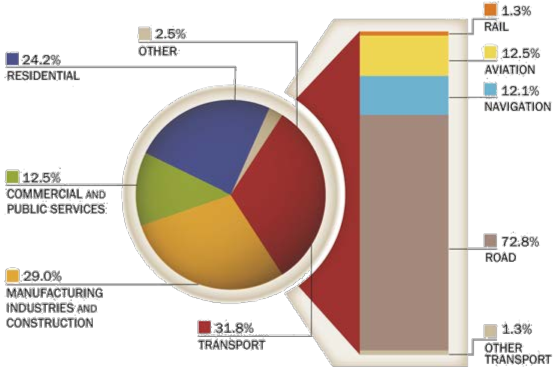
\includegraphics[width=0.93\textwidth,keepaspectratio]{figures/1.Intro/iea-uic-energy}
			\caption{Global Energy Consumption. \cite{iea-uic2016}.}
		\end{figure}
	\end{minipage}\hfill
	\begin{minipage}[t]{0.48\linewidth}
		%\begin{itemize}
		%	\item  50 Hz 25 kV supply system.
		
		%\end{itemize}
		\vspace{4.45em}
		\begin{figure}[ht!]
			\centering
			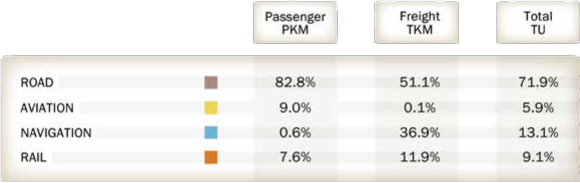
\includegraphics[width=\textwidth,keepaspectratio]{figures/1.Intro/iea-uic-share}
			\caption{Global Transportation Share. \cite{iea-uic2016}.}
		\end{figure}
		
	\end{minipage}
\end{block}
\end{frame}

%%%%%%%%%%%%%%%%%%%%%%%%%%%%%%%%%%%%%%%%%%%%%%%%%%%%%%%%%%%%%%%%%%%%%%%%%%%%%%%%%%%%%

\begin{frame}{Introduction}{Context and motivation of PhD}
\begin{block}{\textbf{Shift2Rail Framework - Main Goal}}
	\begin{itemize}
		%	\setlength\itemsep{-0.5em}
		\item 1. Cutting the life-cycle cost of railway transport by, at least, 50\%;
		\item 2. Doubling the railway capacity;
		\item 3. Increasing the reliability and punctuality by 50\%, at least.
	\end{itemize}
	
\end{block}
\end{frame}
%%%%%%%%%%%%%%%%%%%%%%%%%%%%%%%%%%%%%%%%%%%%%%%%%%%%%%%%%%%%%%%%%%%%%%%%%%%%%%%%%%%%%

\begin{frame}{Introduction}{Context and motivation of PhD}
%\begin{block}{\textbf{Shift2Rail Framework - Time Targets}}
%Complementary, the time target goals are the establishment of a framework, by 2020, for a European multimodal transport system for the passenger rail, freight and for the urban mobility. By 2030 is expected to triple the length of the existing high-speed passenger rail network, 30\% of the road freight over 300 km should shift to rail or waterborne transport and achieve a CO2-free city logistics in major urban centers. By 2050, the medium-distance passenger transport should go by rail and high-speed rail, with the connection of all core network airports to the high-speed railway network. On the freight is expected to have all seaports connected to the rail freight transport system and on the urban mobility, the "conventionally-fueled" cars will not have place in cities by 2050, \cite{shift2rail2015}.
\begin{figure}[ht!]
	\centering
	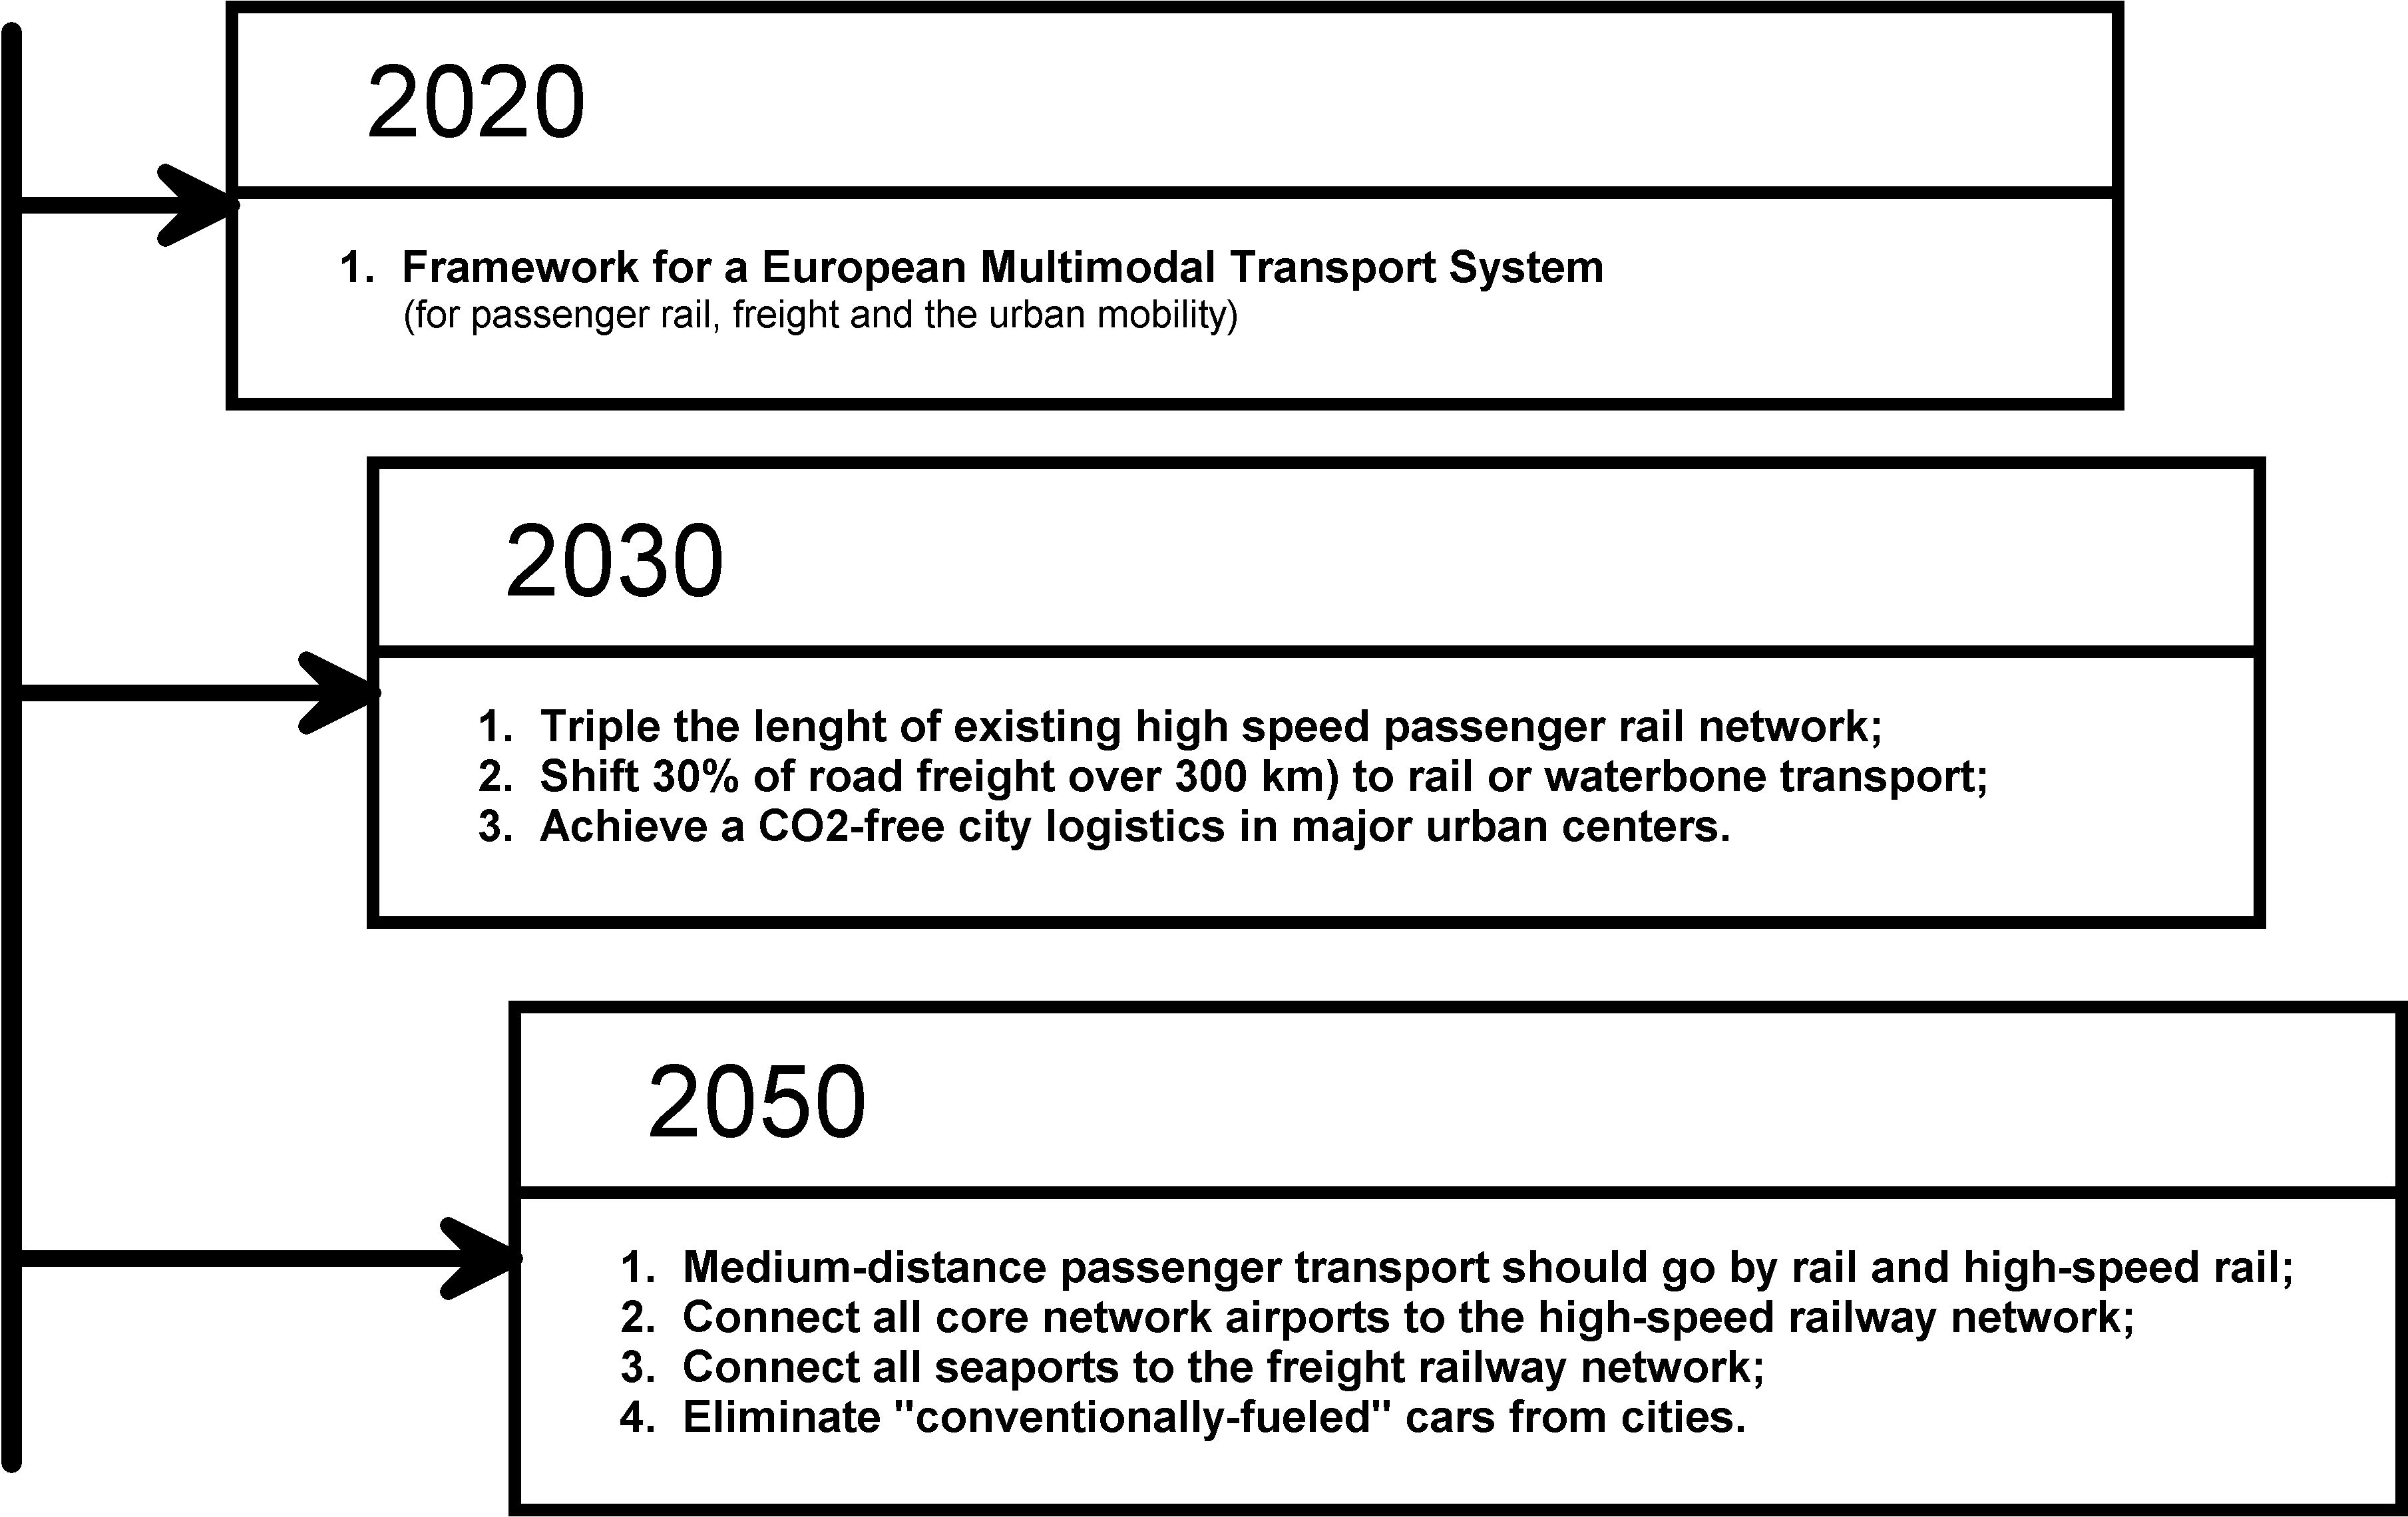
\includegraphics[width=0.7\textwidth,keepaspectratio]{figures/1.Intro/time_targets}
	\caption{Shift2Rail Framework - Time Targets. \cite{shift2rail2015}}
\end{figure}

%\end{block}
\end{frame}
%%%%%%%%%%%%%%%%%%%%%%%%%%%%%%%%%%%%%%%%%%%%%%%%%%%%%%%%%%%%%%%%%%%%%%%%%%%%%%%%%%%%%





\begin{frame}{Introduction}{Context and motivation of PhD}
%\begin{minipage}[t]{0.5\linewidth}
	\begin{figure}[ht!]
	\centering
	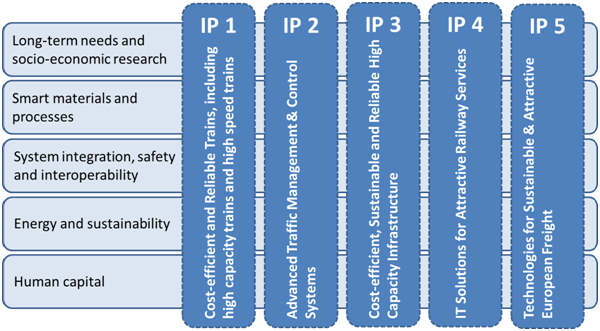
\includegraphics[width=0.6\textwidth,keepaspectratio]{figures/1.Intro/IPs}
	\caption{Shift2Rail Framework - Innovation Programmes. \cite{shift2rail2015}}
	\end{figure}
%\end{minipage}\hfill
%\begin{minipage}[t]{0.48\linewidth}
\vspace{-1em}
	\begin{block}{\textbf{Smart Meter Demonstrator}}
	\begin{itemize}
		\setlength\itemsep{0em}
		\item Towards detailed monitoring and supervision of energy flows;
	\end{itemize}
	\end{block}
	%
		%	The \ac{S2R} carries five innovation programmes, as presented in figure \ref{fig:ips}. Framed on the S2R \ac{IP3} with the focus on the ”Cost efficient and reliable infrastructure”, it is proposed the development of a \ac{SMD} that achieves a detailed monitoring and supervision of various energy flows on the premises of embracing the entire \ac{RTS}.
	%
%\end{minipage}



%\begin{figure}[h!]
%	\centering
%	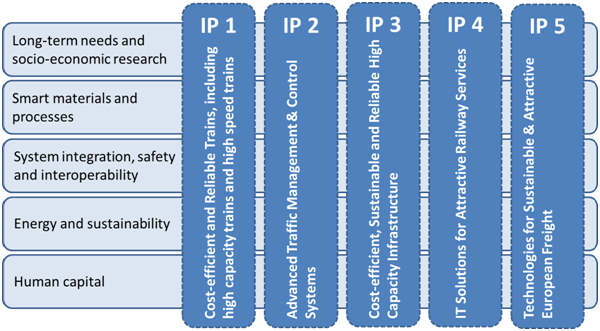
\includegraphics[width=0.60\textwidth,keepaspectratio]{figures/1.Intro/IPs}
%	\caption{Shif2Rail Innovation Programs. }
%\end{figure}
\end{frame}
%%%%%%%%%%%%%%%%%%%%%%%%%%%%%%%%%%%%%%%%%%%%%%%%%%%%%%%%%%%%%%%%%%%%%%%%%%%%%%%%%%%%%

\begin{frame}{Introduction}{Context and motivation of PhD}
%\begin{block}{\textbf{Context and motivation}}
	
	
	\begin{minipage}[t]{0.48\linewidth}
		%\begin{itemize}
		%	\item \ac{DC} supply system architecture	
		%\end{itemize}

		\begin{figure}[ht!]
			\centering
			
\includegraphics[width=0.5\textwidth,keepaspectratio]{figures/1.Intro/grr_magazine_10}
			\caption{Front Page of Global Railway Review magazine.}
		\end{figure}
	\end{minipage}\hfill
	\begin{minipage}[t]{0.48\linewidth}
		%\begin{itemize}
		%	\item  50 Hz 25 kV supply system.
		
		%\end{itemize}
\vspace{2em}
		\begin{figure}[ht!]
			\centering
			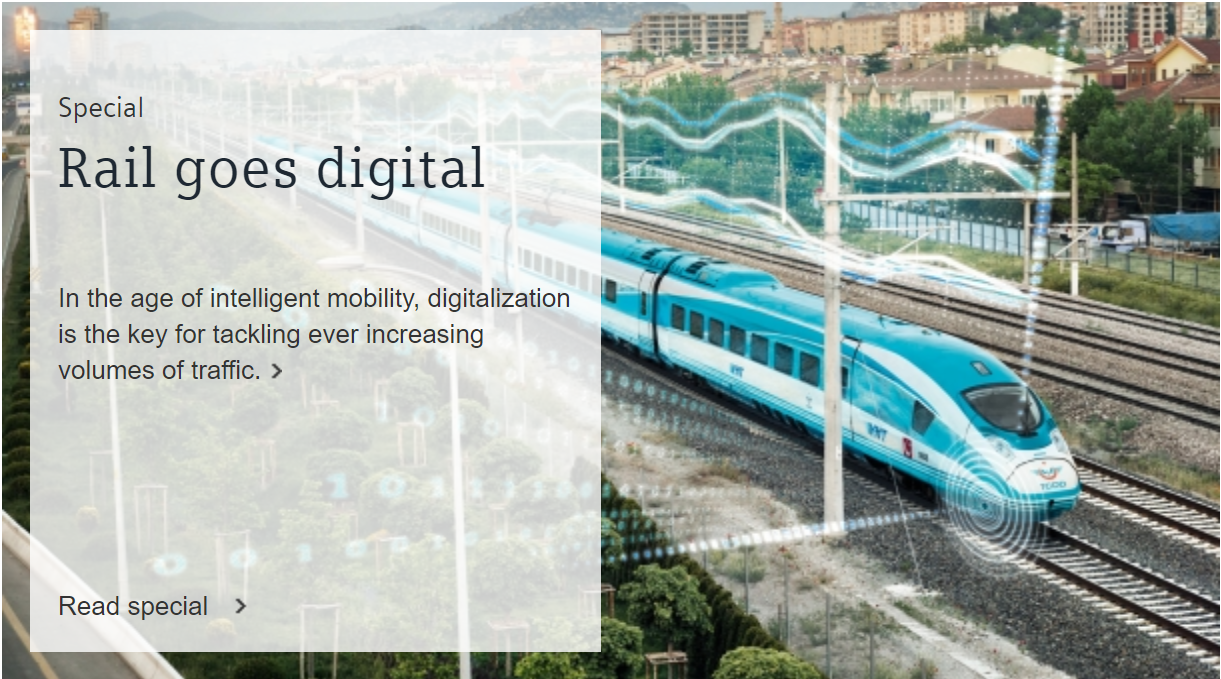
\includegraphics[width=1\textwidth,keepaspectratio]{figures/1.Intro/siemens}
			\caption{Siemens Special Issue in InnoTrans Fair.}
		\end{figure}
		
		
		
	\end{minipage}
	
%\end{block}
\end{frame}
%%%%%%%%%%%%%%%%%%%%%%%%%%%%%%%%%%%%%%%%%%%%%%%%%%%%%%%%%%%%%%%%%%%%%%%%%%%%%%%%%%%%%




%\subsection{Objectives}

\begin{frame}{Introduction}{Objectives}
\begin{block}{\textbf{Objectives}}
\begin{itemize}
	\setlength\itemsep{0em}
	
	\item	Research on \textbf{railway energy models}, and \textbf{development/implementation of a metering system} for railway power flow monitoring.
	This is expected to be based on a non-intrusive self-powered sensor node inserted into train power system.
	
	\item Research on \textbf{communication network models} for a \ac{RTS} wireless network with \textbf{validation through simulation frameworks}.
	\textbf{Development and implementation} of \ac{RTS} wireless network to store the energy information data of railway into central database.
	
	
\end{itemize}
\end{block}
\end{frame}
%%%%%%%%%%%%%%%%%%%%%%%%%%%%%%%%%%%%%%%%%%%%%%%%%%%%%%%%%%%%%%%%%%%%%%%%%%%%%%%%%%%%%

\section{Railway Transportation System}

\subsection{Power system of Railway Transportation System}

\begin{frame}{Power system of Railway Transportation System}
	\begin{block}{\textbf{Overview of Existing European Railway Power Systems}}
	%	Back to the 19th century, the steam turbine was the main propulsion system for the trains. Later on, electric and diesel propulsion systems were adopted. In recent years occurred a massive introduction of power converters based on \ac{IGBT}, which allowed an increase of energy efficiency (allowing, for example, regenerative breaking and reduction of power losses in traction motors).
		
	%	Due to this evolution, different topologies of the railway system exists nowadays. In table \ref{tab:31.t1}, different catenary topologies are visible which results in different power systems for \ac{RTS}.
		
		

			% Table generated by Excel2LaTeX from sheet 'Sheet1'
\begin{table}[htbp]
	\centering
	\tiny
	\caption{Catenary topology and vehicle characteristics of different railway vehicles. \cite{abad2016}.}
	\begin{tabular}{|c|p{10.145em}p{10.355em}|cc|}
		\cmidrule{2-5}    \multicolumn{1}{c|}{} & \multicolumn{2}{c|}{\textbf{Catenary topology}} & \multicolumn{2}{c|}{\textbf{Vehicle characteristics}} \\
		\cmidrule{2-5}    \multicolumn{1}{c|}{} & \multicolumn{1}{c}{\textbf{DC supply}} & \multicolumn{1}{c|}{\textbf{AC supply}} & \textbf{Power} & \textbf{Top speed} \\
		\midrule
		\textbf{Tram} & 600V DC, 750V DC, 900V DC & \multicolumn{1}{c|}{-}     & 150–300kW & 50–70km/h \\
		\midrule
		\textbf{Metro} & 750V DC, 1500V DC & \multicolumn{1}{c|}{-}     & 350kW–1MW & 80km/h \\
		\midrule
		\textbf{Train} & 750V DC, 1500V DC, 3000V DC & 15kV AC (16.7Hz) and 25kV AC (50Hz) & 200kW–8MW & 120–350km/h \\
		\midrule
		\textbf{Locomotive} & 750V DC, 1500V DC, 3000V DC & 15kV AC (16.7Hz) and 25kV AC (50Hz) & 500kW–8MW & 100–200km/h \\
		\bottomrule
	\end{tabular}%
	\label{tab:31.t1}%
\end{table}%


		
	\end{block}
\end{frame}
%%%%%%%%%%%%%%%%%%%%%%%%%%%%%%%%%%%%%%%%%%%%%%%%%%%%%%%%%%%%%%%%%%%%%%%%%%%%%%%%%%%%%

\begin{frame}{Railway Transportation System}{Power system of Railway Transportation System}
%\begin{block}{\textbf{Overview of Existing European Railway Power Systems}}


\begin{figure}[h!]
	\centering
	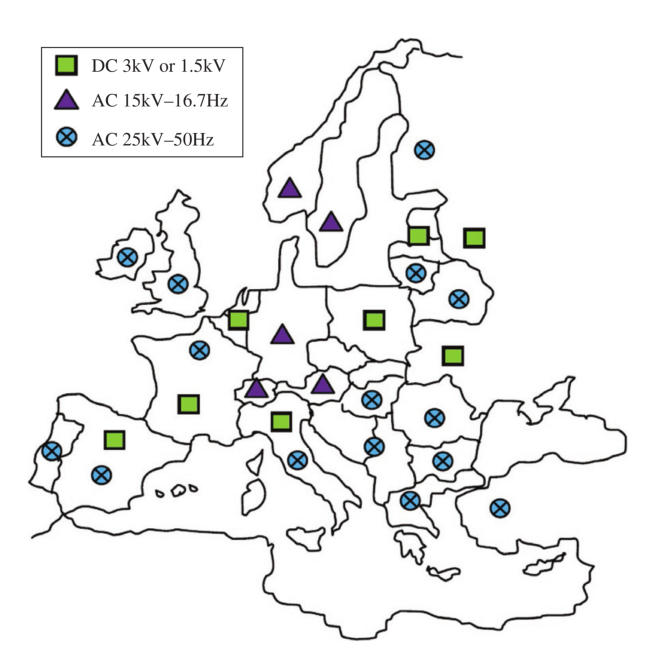
\includegraphics[width=0.4\textwidth,keepaspectratio]{figures/31.PowerS/abad2016}
	\caption{Railway main-line power supply systems in Europe. \cite{abad2016}.}
	\label{fig:abad2016}
\end{figure}
	
	
%\end{block}
\end{frame}
%%%%%%%%%%%%%%%%%%%%%%%%%%%%%%%%%%%%%%%%%%%%%%%%%%%%%%%%%%%%%%%%%%%%%%%%%%%%%%%%%%%%%

%\subsection{Railway Power Supply System}


\begin{frame}{Railway Transportation System}{Power system of Railway Transportation System}
	\begin{minipage}[t]{0.48\linewidth}
	%\begin{itemize}
	%	\item \ac{DC} supply system architecture	
	%\end{itemize}
	
	\begin{figure}[ht!]
		\centering
		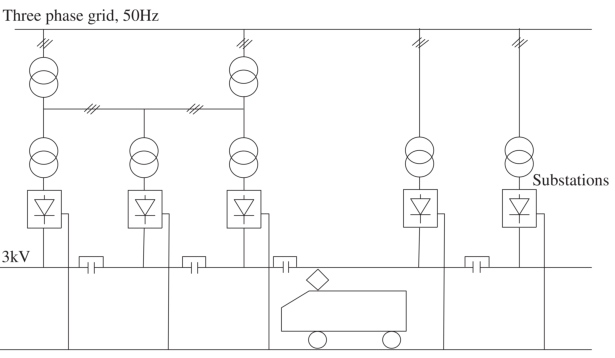
\includegraphics[width=0.7\textwidth,keepaspectratio]{figures/31.PowerS/abad2016f}
		\caption{\ac{DC} supply system architecture. \cite{abad2016}.}
	\end{figure}
\end{minipage}\hfill
\begin{minipage}[t]{0.48\linewidth}
	%\begin{itemize}
	%	\item  50 Hz 25 kV supply system.
	
	%\end{itemize}
	
	\begin{figure}[ht!]
		\centering
		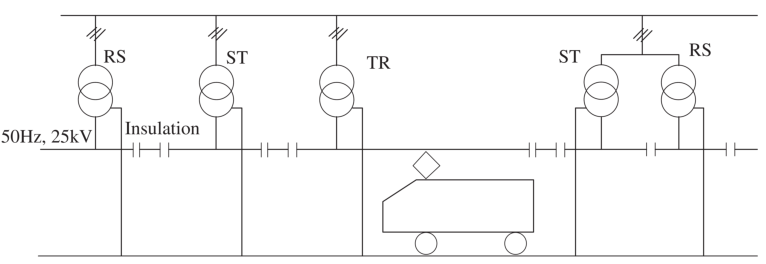
\includegraphics[width=\textwidth,keepaspectratio]{figures/31.PowerS/abad2016d}
		\caption{50 Hz 25 kV supply system. \cite{abad2016}.}
	\end{figure}


	
\end{minipage}

\begin{minipage}[t]{0.24\linewidth} ~ \end{minipage}
\begin{minipage}[t]{0.48\linewidth}

\begin{figure}[ht!]
	\centering
	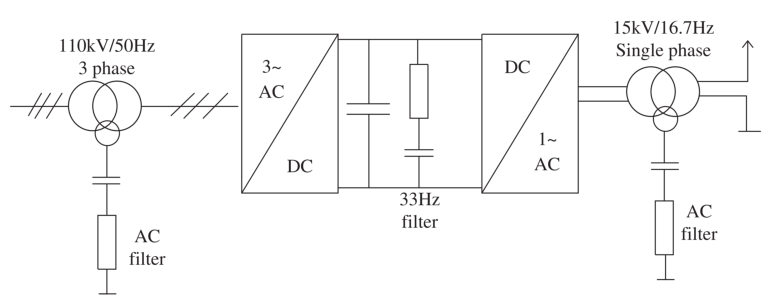
\includegraphics[width=\textwidth,keepaspectratio]{figures/31.PowerS/abad2016e}
	\caption{16.7 Hz 15 kV supply system. \cite{abad2016}.}
\end{figure}
\end{minipage}

\end{frame}
%%%%%%%%%%%%%%%%%%%%%%%%%%%%%%%%%%%%%%%%%%%%%%%%%%%%%%%%%%%%%%%%%%%%%%%%%%%%%%%%%%%%%

\subsection{Train Power Supply System}

\begin{frame}{Railway Transportation System}{Train Power Supply System}
%\begin{block}{\textbf{Overview of Existing European Railway Power Systems}}


\begin{figure}[h!]
	\centering
	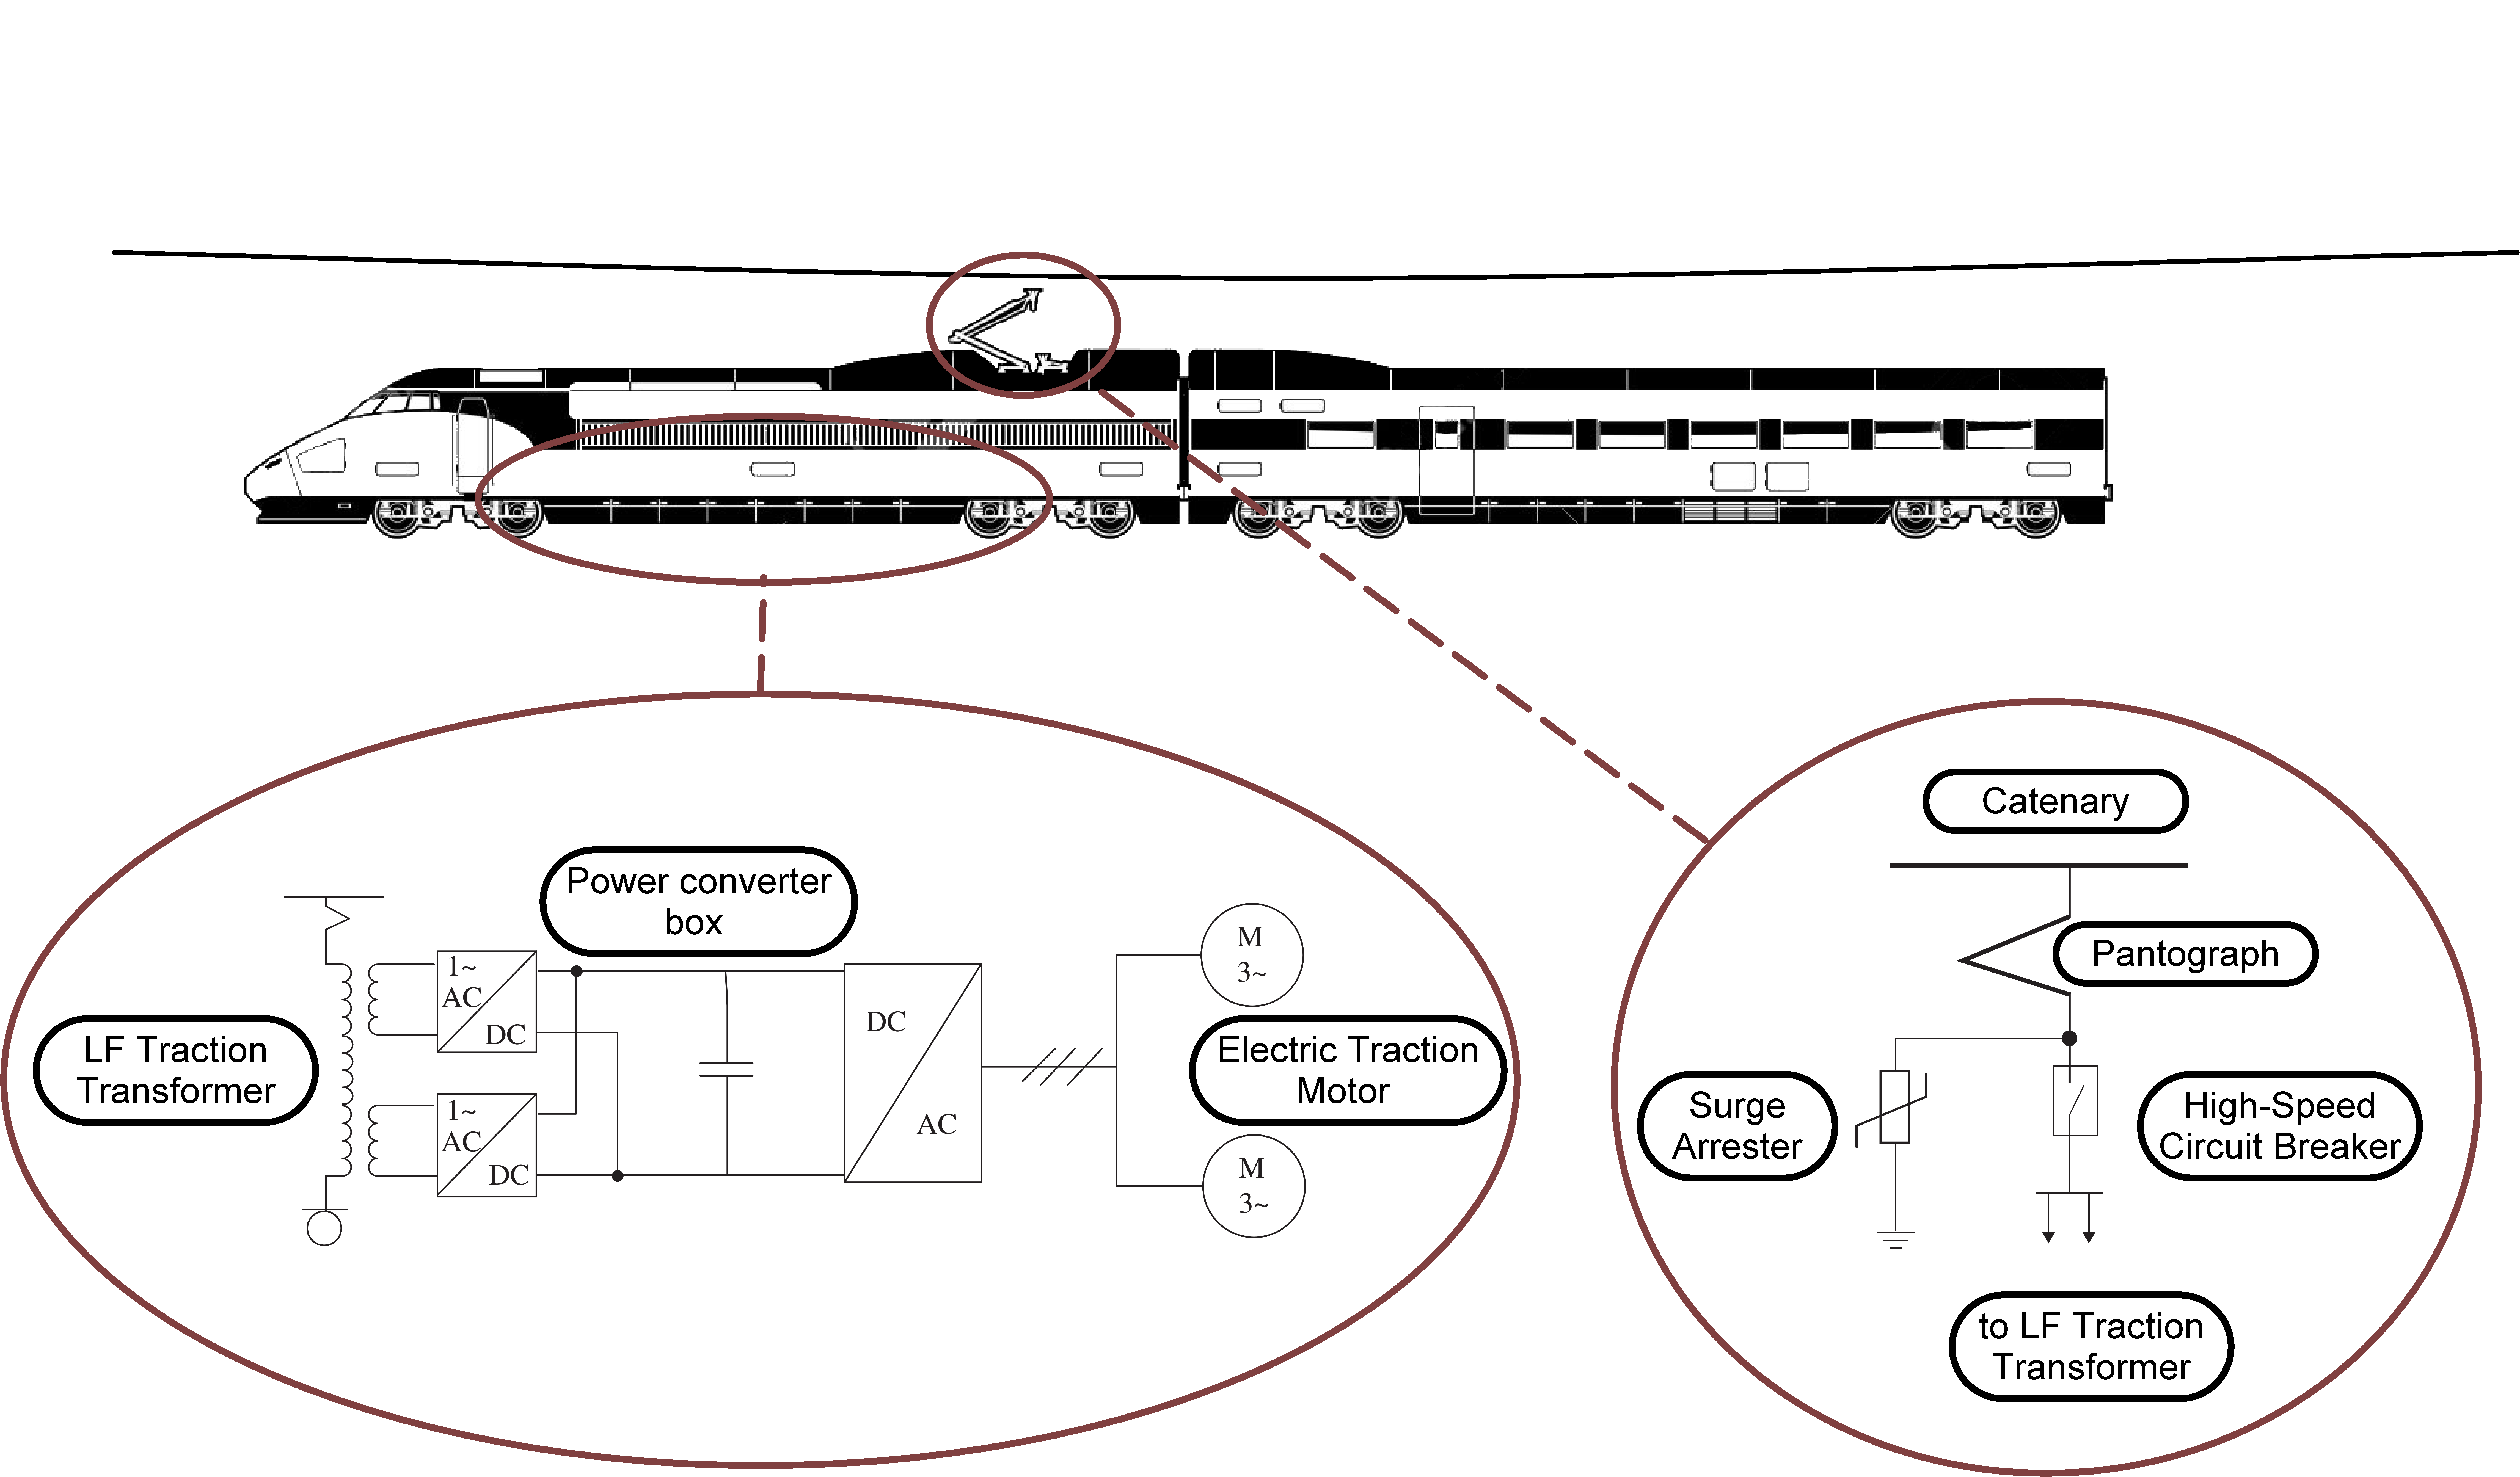
\includegraphics[width=0.85\textwidth,keepaspectratio]{figures/31.PowerS/train_finale}
	\caption{Train Power Components.}
	\label{fig:abad2016}
\end{figure}


%\end{block}
\end{frame}
%%%%%%%%%%%%%%%%%%%%%%%%%%%%%%%%%%%%%%%%%%%%%%%%%%%%%%%%%%%%%%%%%%%%%%%%%%%%%%%%%%%%%

\begin{frame}{Railway Transportation System}{Train Power Supply System}
%\begin{block}{\textbf{Overview of Existing European Railway Power Systems}}


	\begin{minipage}[t]{0.48\linewidth}

	
	\begin{figure}[ht!]
		\centering
			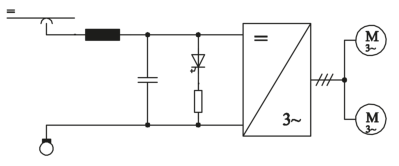
\includegraphics[width=0.8\textwidth,keepaspectratio]{figures/31.PowerS/steimel2008a}
		%		\vspace{0.5em}
		\caption{Train internal power circuit of a \ac{DC} supply system. Adapted from \cite{steimel2008}.}
	\end{figure}
\end{minipage}\hfill
\begin{minipage}[t]{0.48\linewidth}
	%\begin{itemize}
	%	\item  50 Hz 25 kV supply system.
	
	%\end{itemize}
	
	\begin{figure}[ht!]
		\centering
		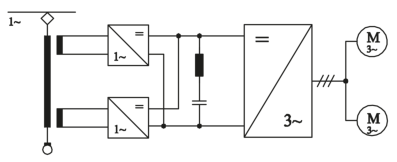
\includegraphics[width=0.8\textwidth,keepaspectratio]{figures/31.PowerS/steimel2008b}
		%		\vspace{0.5em}
		\caption{Train internal power circuit of an \ac{AC} supply system. Adapted from \cite{steimel2008}.}
	\end{figure}
	
	
	
\end{minipage}

\begin{minipage}[t]{0.24\linewidth} ~ \end{minipage}
\begin{minipage}[t]{0.48\linewidth}
	
	\begin{figure}[ht!]
		\centering
		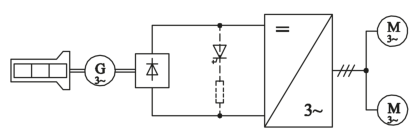
\includegraphics[width=0.8\textwidth,keepaspectratio]{figures/31.PowerS/steimel2008c}
		\caption{Train internal power circuit of a Diesel electric locomotive with alternator. Adapted from \cite{steimel2008}.}
	\end{figure}
\end{minipage}

%\end{block}
\end{frame}
%%%%%%%%%%%%%%%%%%%%%%%%%%%%%%%%%%%%%%%%%%%%%%%%%%%%%%%%%%%%%%%%%%%%%%%%%%%%%%%%%%%%%

\begin{frame}{Railway Transportation System}
\begin{block}{\textbf{Case study --- Series 3400 train}}

	\begin{minipage}[t]{0.48\linewidth}
		
		
		\begin{figure}[ht!]
			\centering
			\includegraphics[width=0.85\textwidth,keepaspectratio]{figures/40.Method/powerSensing}
			%		\vspace{0.5em}
			\caption{Power architecture of case study train.}
		\end{figure}
	\end{minipage}\hfill
	\begin{minipage}[t]{0.48\linewidth}
		%\begin{itemize}
		%	\item  50 Hz 25 kV supply system.
		
		%\end{itemize}
		
		\begin{figure}[ht!]
			\centering
					\vspace{2em}
			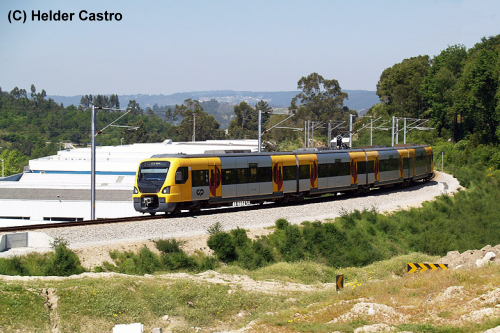
\includegraphics[width=0.95\textwidth,keepaspectratio]{figures/40.Method/CP3400}
			%		\vspace{0.5em}
			\caption{Series 3400 case study train. Retrieved from \textit{Comboios de Portugal}}
		\end{figure}
		
		
		
	\end{minipage}
	
	
\end{block}
\end{frame}

\section{Remote Monitoring in Railways}

\subsection{Energy sensors}

\begin{frame}{Remote Monitoring in Railways}{Energy sensors}
	\begin{block}{\textbf{Transducers}}
	
	\begin{minipage}[t]{0.48\linewidth}
		\vspace{5em}
	\begin{itemize}
		\item Magnetic Coupling
		\item Magneto Resistance
		\item Faraday Induction
		\item Hall Effect
	\end{itemize}
	\end{minipage}\hfill
	\begin{minipage}[t]{0.48\linewidth}
		%\begin{itemize}
		%	\item  50 Hz 25 kV supply system.
		
		%\end{itemize}
		
		\begin{figure}[ht!]
			\centering
			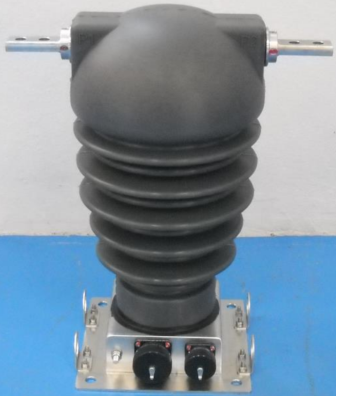
\includegraphics[width=0.30\textwidth,keepaspectratio]{figures/32.EnergyS/current_t}
			\caption{25 kV current transformer. Adapted from \textit{www.railware.it}}
		\end{figure}
		
			\begin{figure}[ht!]
			\centering
			\vspace{-3em}
			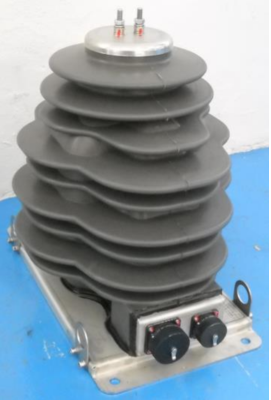
\includegraphics[width=0.25\textwidth,keepaspectratio]{figures/32.EnergyS/voltage_t}
			\caption{25 kV voltage transformer. Adapted from \textit{www.railware.it}}
		\end{figure}
		
		
	\end{minipage}
	

		
	\end{block}
\end{frame}
%%%%%%%%%%%%%%%%%%%%%%%%%%%%%%%%%%%%%%%%%%%%%%%%%%%%%%%%%%%%%%%%%%%%%%%%%%%%%%%%%%%%%

\begin{frame}{Remote Monitoring in Railways}{Energy Sensors --- Power Calculation Function}
%\begin{block}{\textbf{Overview of Existing European Railway Power Systems}}


\begin{figure}[h!]
	\centering
	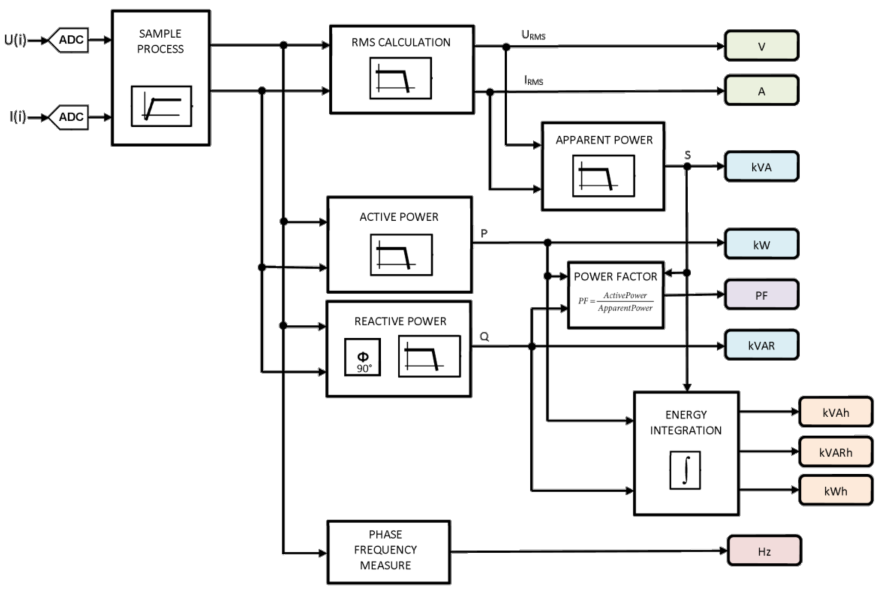
\includegraphics[width=0.7\textwidth,keepaspectratio]{figures/32.EnergyS/energy_calculation}
	\caption{EcoS power calculation function, based on EN50463. Adapted from railware.it}
\end{figure}
	
	
%\end{block}
\end{frame}
%%%%%%%%%%%%%%%%%%%%%%%%%%%%%%%%%%%%%%%%%%%%%%%%%%%%%%%%%%%%%%%%%%%%%%%%%%%%%%%%%%%%%

\subsection{Wireless Networks}

\begin{frame}{Remote Monitoring in Railways}{Wireless Networks}

\begin{figure}[h!]
	\centering
	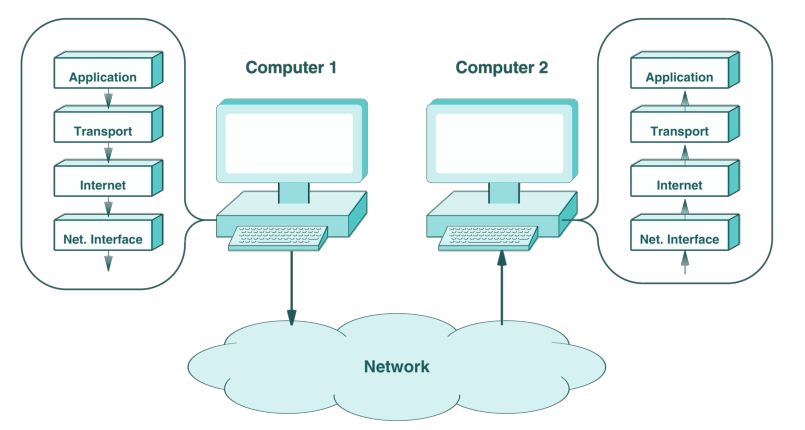
\includegraphics[width=0.8\textwidth,keepaspectratio]{figures/33.WirelessN/comer2008}
	\caption{Representation of data flow in a computer network. Adapted from \cite{comer2008}.}
\end{figure}

\end{frame}
%%%%%%%%%%%%%%%%%%%%%%%%%%%%%%%%%%%%%%%%%%%%%%%%%%%%%%%%%%%%%%%%%%%%%%%%%%%%%%%%%%%%%


\begin{frame}{Remote Monitoring in Railways}{Wireless Networks --- Simulators}
\begin{block}{\textbf{Wireless Networks --- Simulators}}
	
	\begin{minipage}[t]{0.48\linewidth}
	%	\vspace{5em}
		\begin{itemize}
			\item NS-3
			\item OMNeT++
			\item QualNet 7.0 + EXata 5
			\item MatLab + Simulink
		\end{itemize}
	\end{minipage}\hfill
	\begin{minipage}[t]{0.48\linewidth}
		
		\begin{figure}[ht!]
			\centering
			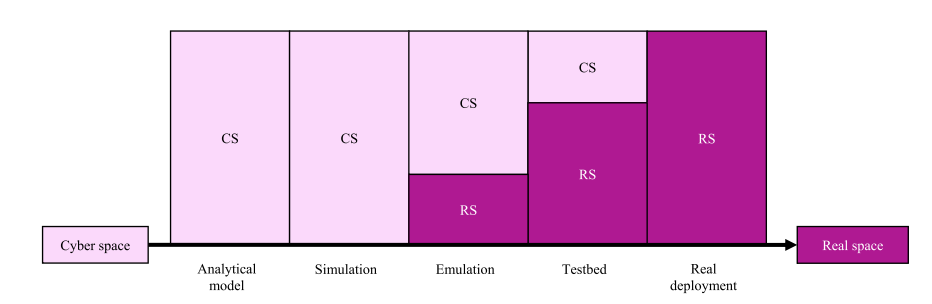
\includegraphics[width=1\textwidth,keepaspectratio]{figures/33.WirelessN/simul_VS_emul}
			\caption{Simulation \& emulation framework.}
		\end{figure}
	
	\end{minipage}
	
	
	
\end{block}
\end{frame}
%%%%%%%%%%%%%%%%%%%%%%%%%%%%%%%%%%%%%%%%%%%%%%%%%%%%%%%%%%%%%%%%%%%%%%%%%%%%%%%%%%%%%

%%%%%%%%%%%%%%%%%%%%%%%%%%%%%%%%%%%%%%%%%%%%%%%%%%%%%%%%%%%%%%%%%%%%%%%%%%%%%%%%%%%%%

\subsection{Smart metering in railways}

\begin{frame}{Remote Monitoring in Railways}{Smart metering in railways}

\begin{figure}[h!]
	\centering
		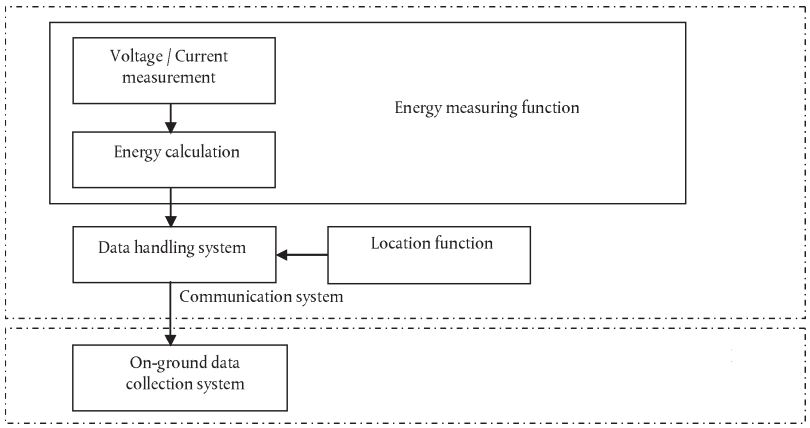
\includegraphics[width=0.8\textwidth,keepaspectratio]{figures/34.SmartM/EMS}
	\caption{Functions, data flow and regulation scope of on-board energy measurement system.}
\end{figure}

\end{frame}
%%%%%%%%%%%%%%%%%%%%%%%%%%%%%%%%%%%%%%%%%%%%%%%%%%%%%%%%%%%%%%%%%%%%%%%%%%%%%%%%%%%%%

\subsection{Decision Support Systems}
%%%%%%%%%%%%%%%%%%%%%%%%%%%%%%%%%%%%%%%%%%%%%%%%%%%%%%%%%%%%%%%%%%%%%%%%%%%%%%%%%%%%%


\begin{frame}{Remote Monitoring in Railways}{Decision Support Systems}
\begin{block}{\textbf{Decision Support Systems}}
	
	\begin{minipage}[t]{0.48\linewidth}
		%	\vspace{5em}
		\begin{itemize}
			\item Eco-driving --- Driving Assistant
			\item Timetable Scheduling
		\end{itemize}
	\end{minipage}\hfill
	\begin{minipage}[t]{0.48\linewidth}
		
		\begin{figure}[ht!]
			\centering
			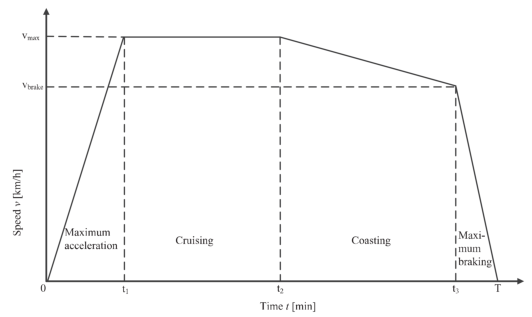
\includegraphics[width=0.5\textwidth,keepaspectratio]{figures/35.DSS/scheepmaker2017a}
			\caption{Optimal traction regimes. Adapted from \cite{scheepmaker2017}.}
		\end{figure}
		
	\end{minipage}

\end{block}
\end{frame}
%%%%%%%%%%%%%%%%%%%%%%%%%%%%%%%%%%%%%%%%%%%%%%%%%%%%%%%%%%%%%%%%%%%%%%%%%%%%%%%%%%%%%

\subsection{Issues and problems in Wireless Networks}
%%%%%%%%%%%%%%%%%%%%%%%%%%%%%%%%%%%%%%%%%%%%%%%%%%%%%%%%%%%%%%%%%%%%%%%%%%%%%%%%%%%%%


\begin{frame}{Issues and problems in Wireless Networks}{Outlier Detection Techniques}
\begin{block}{\textbf{Outlier Detection Techniques for RTS}}
	
	\begin{minipage}[t]{0.6\linewidth}
		%	\vspace{5em}
		\begin{itemize}
			%\setlength\itemsep{-0.5em}
			\footnotesize
			\item \textbf{Classification based techniques.}
			\begin{itemize}
				\item Bayesian Networks
				\item Rule-based techniques
				\item Support Vector Machines
			\end{itemize}
			
			\item \textbf{Statistical based techniques.}
			\begin{itemize}
				\item Parametric --- Gaussian based
				\item Non-parametric --- Histogram based
				\item Non-parametric --- Kernel function based
			\end{itemize}
		
			\item \textbf{Nearest Neighbor-based techniques.}
			\begin{itemize}
				\item Using distance
				\item Using relative density
			\end{itemize}
			\item \textbf{Clustering based techniques.}
			
			\item \textbf{Spectral Decomposition based techniques.}
			
		\end{itemize}
	\end{minipage}\hfill
	\begin{minipage}[t]{0.38\linewidth}
		
		\begin{figure}[ht!]
			\centering
			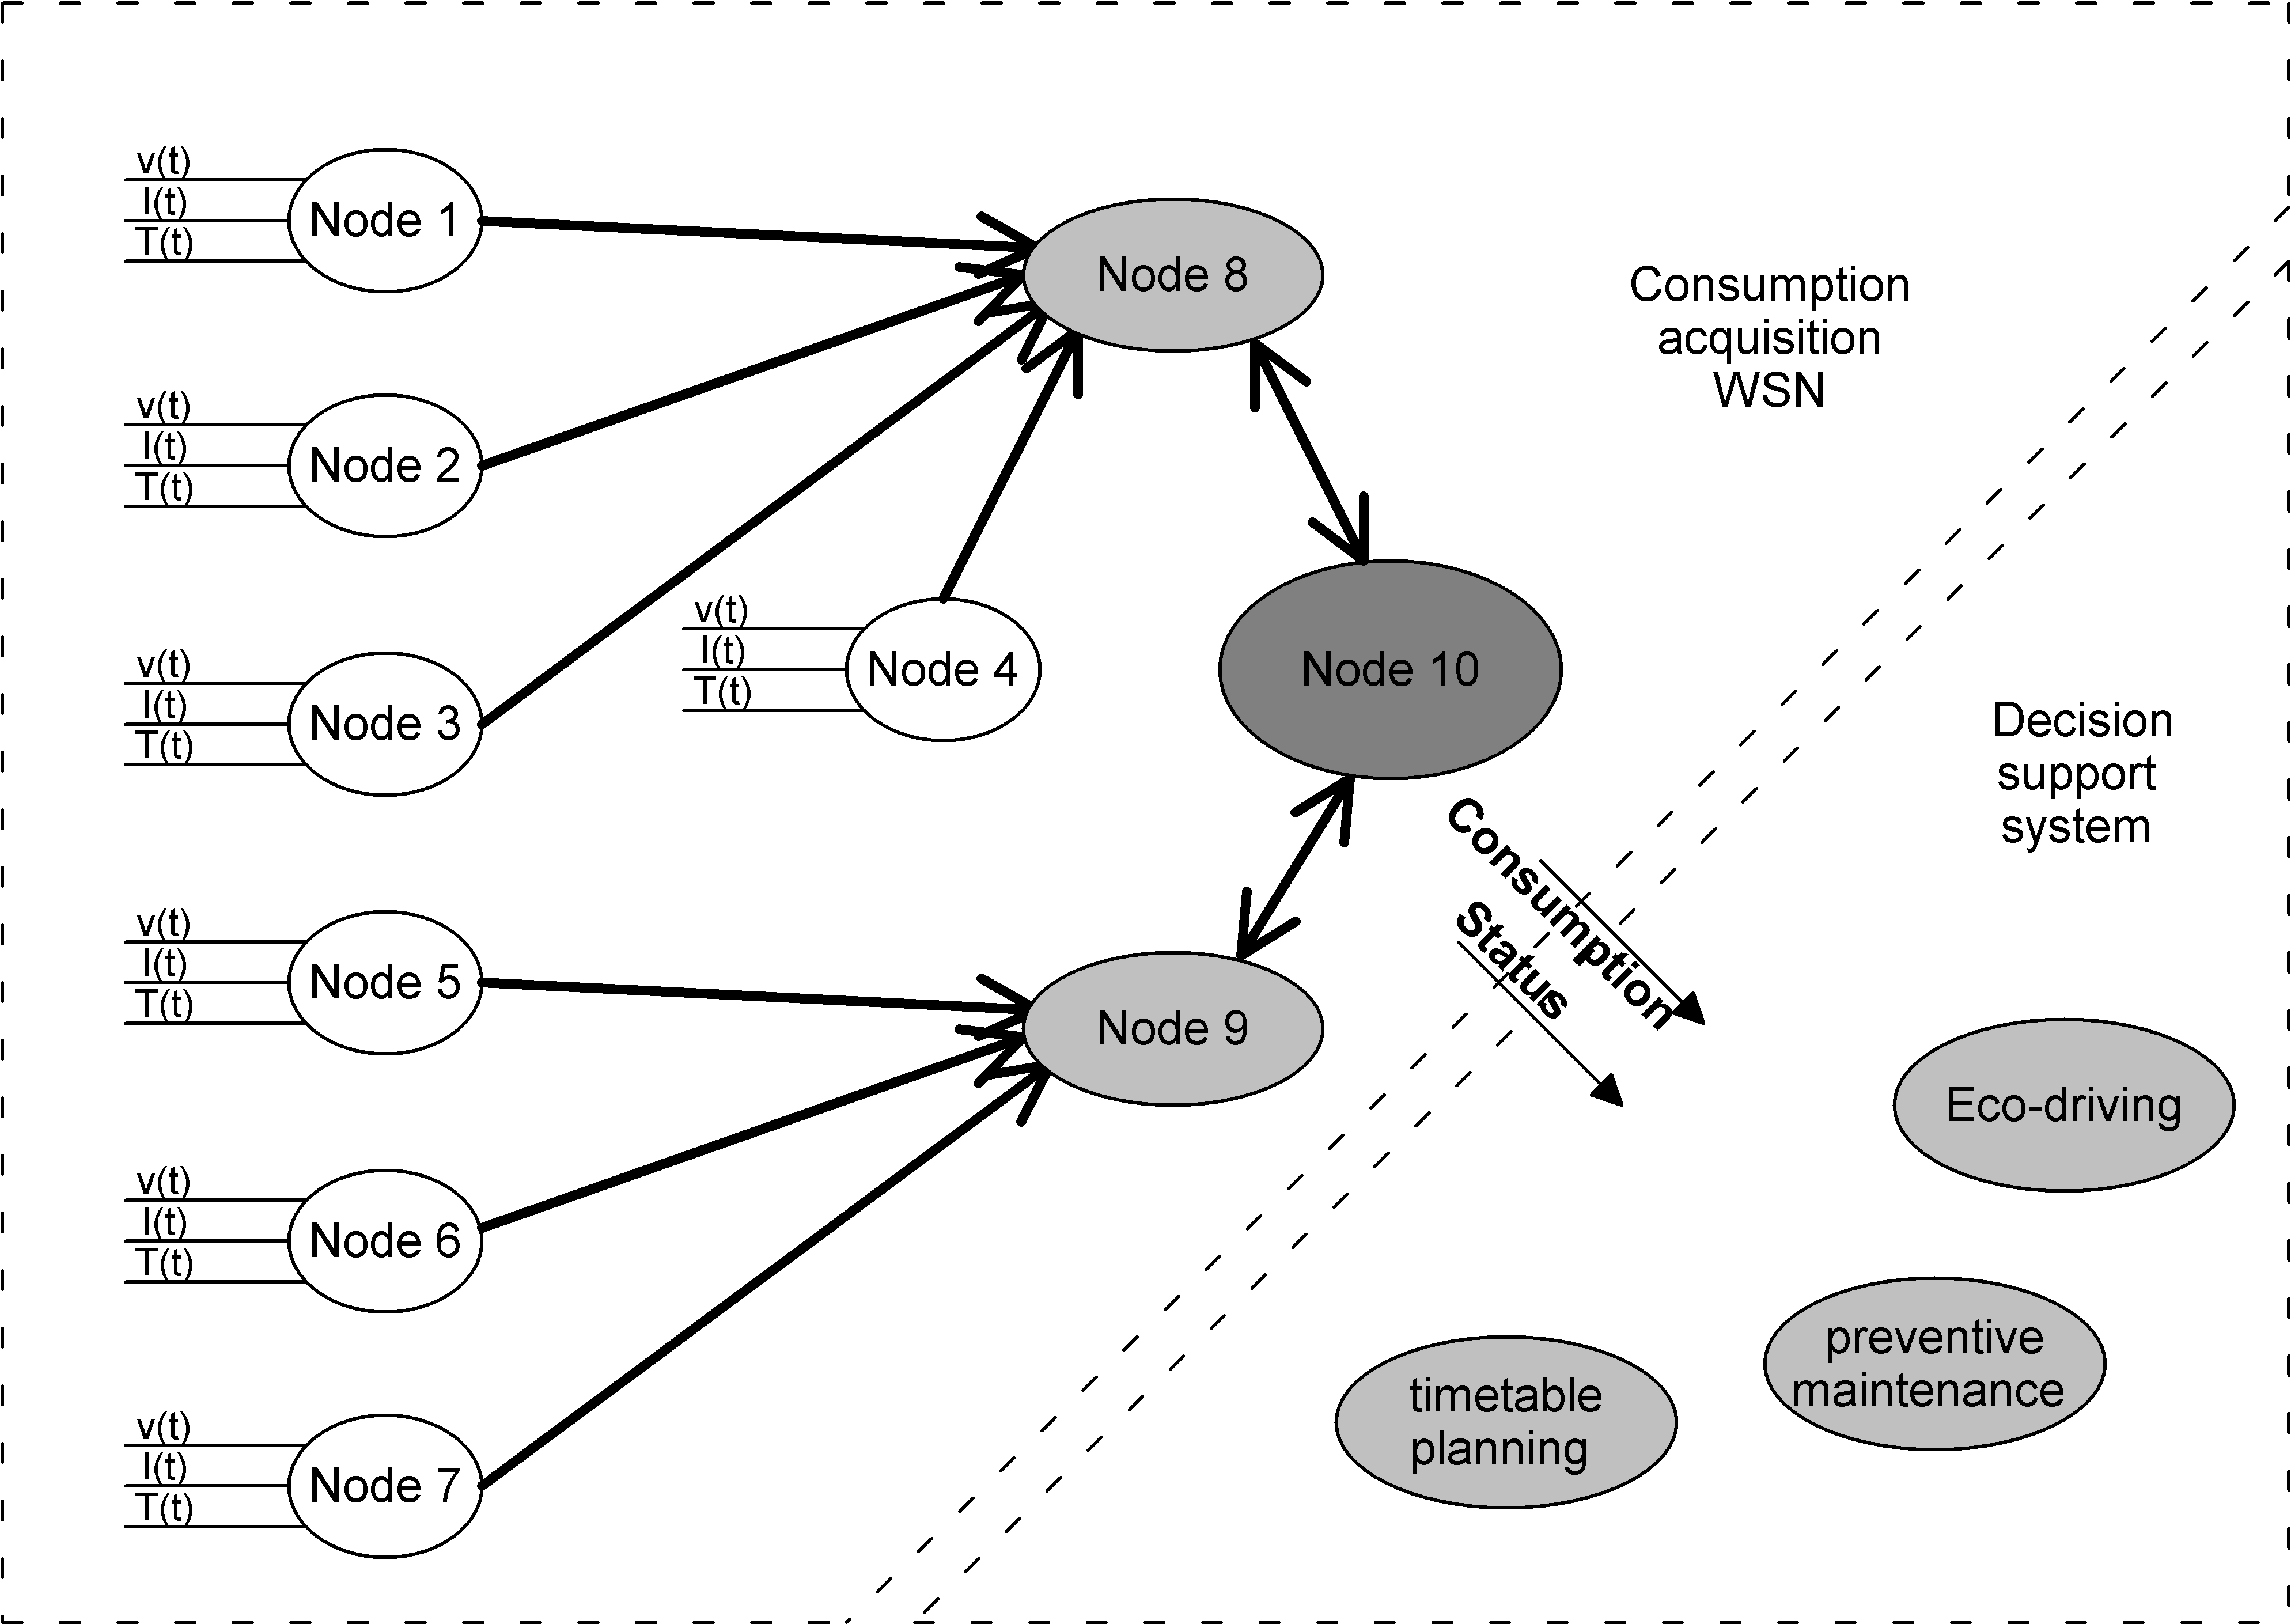
\includegraphics[width=0.95\textwidth,keepaspectratio]{figures/36.Outlier/general}
			\caption{Integration of the \ac{WSN} with a decision support system. }
		\end{figure}
		
	\end{minipage}
	
\end{block}
\end{frame}
%%%%%%%%%%%%%%%%%%%%%%%%%%%%%%%%%%%%%%%%%%%%%%%%%%%%%%%%%%%%%%%%%%%%%%%%%%%%%%%%%%%%%

\section{Thesis Proposal}

\subsection{Architecture of proposed work}

\begin{frame}{Thesis Proposal}{Architecture of proposed work}
\begin{block}{\textbf{Architecture of proposed work}}
	
	\begin{minipage}[t]{0.48\linewidth}
		
		\vspace{2em}
		\begin{figure}[ht!]
			\centering
			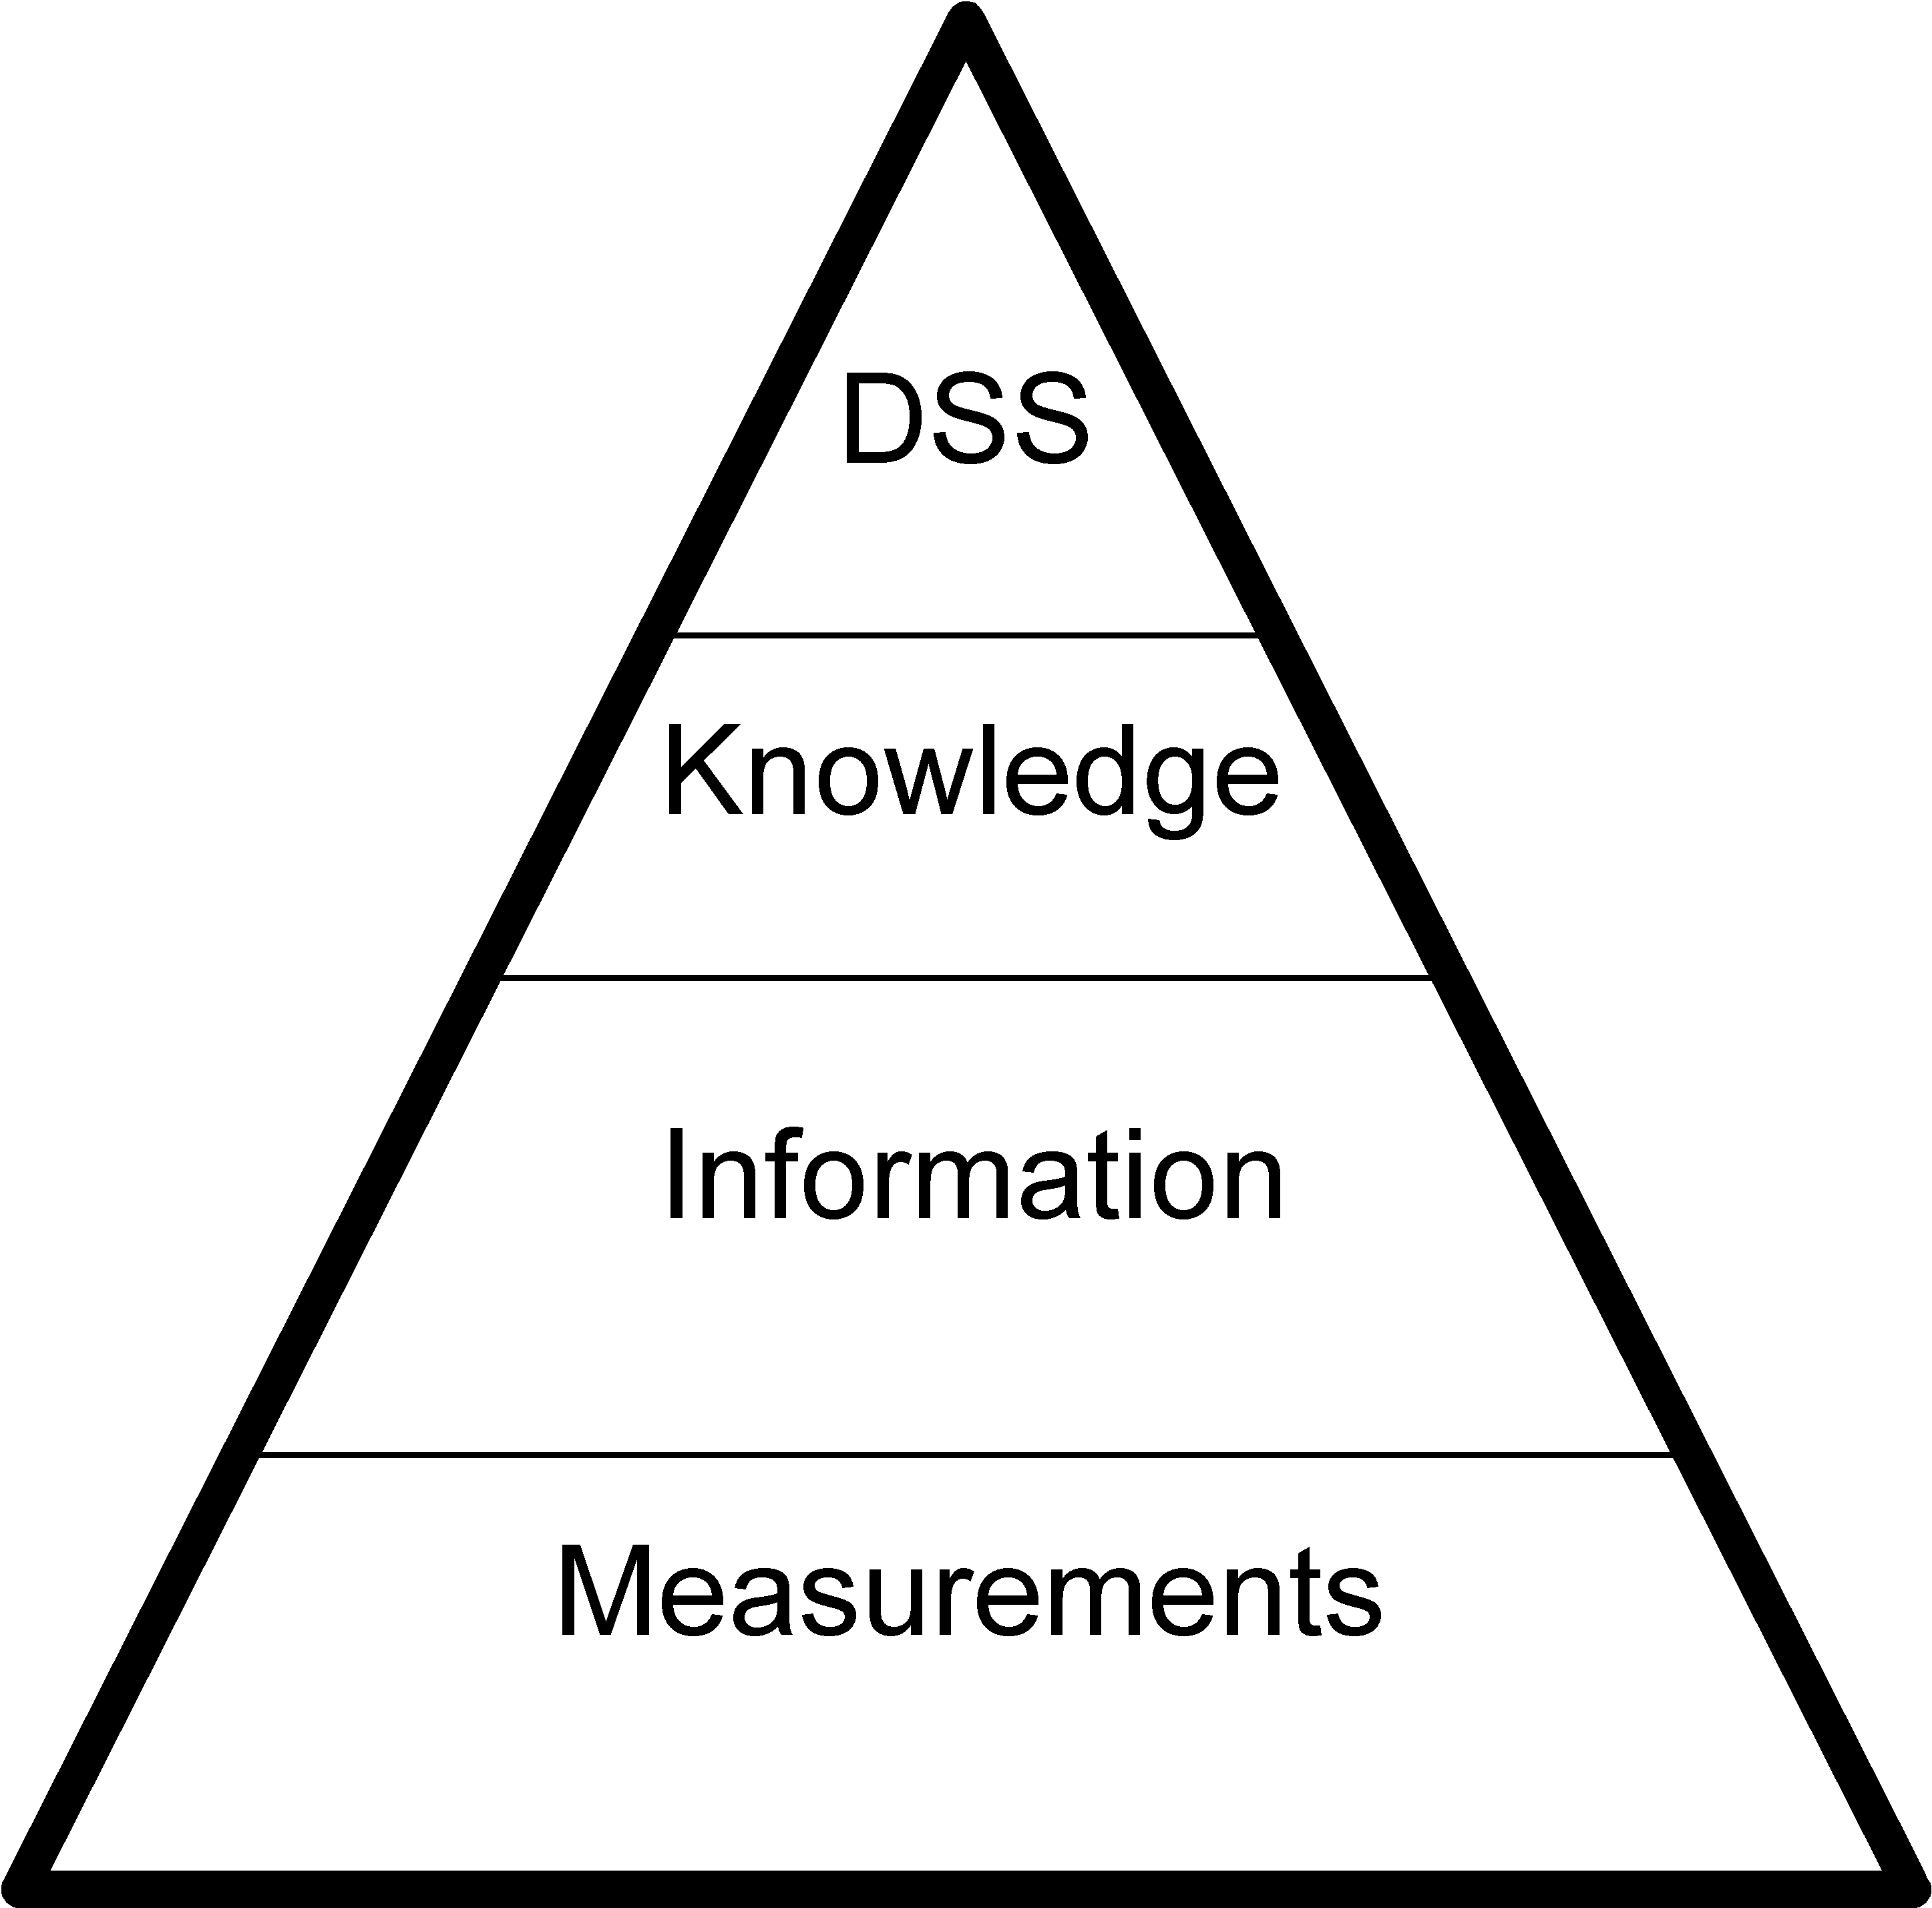
\includegraphics[width=0.4\textwidth,keepaspectratio]{figures/40.Method/pyramid}
			\caption{Overall functional architecture of a smart metering system.}
		\end{figure}

	\end{minipage}\hfill
	\begin{minipage}[t]{0.48\linewidth}
		
		\vspace{2em}
		\begin{figure}[ht!]
			\centering

			
\includegraphics[width=\textwidth,keepaspectratio]{figures/40.Method/data_flow}
			\caption{Data flow of measurement-information layers.}
		\end{figure}
	\hfill
	\vspace{-2em}
		\begin{itemize}
		\item  Non-intrusive self-powered sensor node;
		\item  RTS wireless network
	\end{itemize}
		
	
		
	\end{minipage}
	
\end{block}
\end{frame}
%%%%%%%%%%%%%%%%%%%%%%%%%%%%%%%%%%%%%%%%%%%%%%%%%%%%%%%%%%%%%%%%%%%%%%%%%%%%%%%%%%%%%

\begin{frame}{Thesis Proposal}{Architecture of proposed work}

	\begin{figure}[ht!]
		\centering
		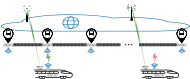
\includegraphics[width=0.9\textwidth,keepaspectratio]{figures/40.Method/architecture}
		\caption{Architecture of proposed work.}
	\end{figure}
		

\end{frame}
%%%%%%%%%%%%%%%%%%%%%%%%%%%%%%%%%%%%%%%%%%%%%%%%%%%%%%%%%%%%%%%%%%%%%%%%%%%%%%%%%%%%%


\subsection{Non-intrusive self-powered sensor node}


\begin{frame}{Thesis Proposal}{Non-intrusive self-powered sensor node}
\begin{block}{\textbf{Non-intrusive self-powered sensor node}}
	\begin{figure}[ht!]
		\centering
		\includegraphics[width=0.5\textwidth,keepaspectratio]{figures/40.Method/powerSensing}
		\caption{Power architecture of case-study train.}
	\end{figure}
\end{block}
\end{frame}
%%%%%%%%%%%%%%%%%%%%%%%%%%%%%%%%%%%%%%%%%%%%%%%%%%%%%%%%%%%%%%%%%%%%%%%%%%%%%%%%%%%%%

\begin{frame}{Thesis Proposal}{Non-intrusive self-powered sensor node}
\begin{block}{\textbf{Non-intrusive self-powered sensor node --- Methodology}}

	\begin{figure}[ht!]
		\centering
		\includegraphics[width=0.7\textwidth,keepaspectratio]{figures/40.Method/methodElectrical}
		\caption{Models needed for simulation. Energy measurement system.}
	\end{figure}

\end{block}
\end{frame}
%%%%%%%%%%%%%%%%%%%%%%%%%%%%%%%%%%%%%%%%%%%%%%%%%%%%%%%%%%%%%%%%%%%%%%%%%%%%%%%%%%%%%

\begin{frame}{Thesis Proposal}{Non-intrusive self-powered sensor node}
\begin{block}{\textbf{Non-intrusive self-powered sensor node --- Contributions}}
		\begin{itemize}
			\item \textbf{New energy metering architecture}, according to some specifications such as the usage of a non-intrusive approach.
			This architecture will generate energy information about the power flow of the railway system.
			
			\item \textbf{Accurate estimation of power flow} into catenary, based on on-board measurements. The available parameters will be: (1) the RMS voltage, current and apparent power, (2) the instantaneous active power, reactive power, power factor and frequency, and (3) the cumulative energy consumptions in terms of kVAh, kVARh and KWh.
		\end{itemize}
\end{block}
\end{frame}


\subsection{RTS wireless network}


\begin{frame}{Thesis Proposal}{RTS wireless network}
\begin{block}{\textbf{RTS wireless network}}
\begin{figure}[ht!]
	\centering
	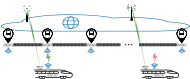
\includegraphics[width=0.8\textwidth,keepaspectratio]{figures/40.Method/architecture}
	\caption{Architecture of proposed work.}
\end{figure}
\end{block}
\end{frame}
%%%%%%%%%%%%%%%%%%%%%%%%%%%%%%%%%%%%%%%%%%%%%%%%%%%%%%%%%%%%%%%%%%%%%%%%%%%%%%%%%%%%%

\begin{frame}{Thesis Proposal}{RTS wireless network}
\begin{block}{\textbf{RTS wireless network --- Methodology}}

\begin{figure}[ht!]
	\centering
	\includegraphics[width=0.8\textwidth,keepaspectratio]{figures/40.Method/methodWireless}
	\caption{Models needed for simulation - RTS Wireless Network.}
\end{figure}

\end{block}
\end{frame}
%%%%%%%%%%%%%%%%%%%%%%%%%%%%%%%%%%%%%%%%%%%%%%%%%%%%%%%%%%%%%%%%%%%%%%%%%%%%%%%%%%%%%

\begin{frame}{Thesis Proposal}{RTS wireless network}
\begin{block}{\textbf{RTS wireless network --- Contributions}}
\begin{itemize}
\item \textbf{Availability of measured data} from trains where currently limited/inexistent energy measurement is performed.

\item Data-rate increase of energy measurements, which will result on direct \textbf{increase on the quality of information of energy}. This increase will overcome the 5-minute data-rate that currently are used in energy meters.

\item A further contribution can be the reduction of the dependence of broadband real-time/continuous communication (such as \ac{LTE}), with the direct cost reduction of information transmission of energy \ac{RTS} data.
\end{itemize}
\end{block}
\end{frame}


\section{Preliminary Work}

\subsection{Implementation of a point-to-point communication between a moving train and a station}

\begin{frame}{Preliminary Work}{Implementation of a point-to-point communication between a moving train and a station}
\begin{block}{\textbf{Implementation of a point-to-point communication between a moving train and a station}}
	
	\begin{figure}[ht!]
		\centering
			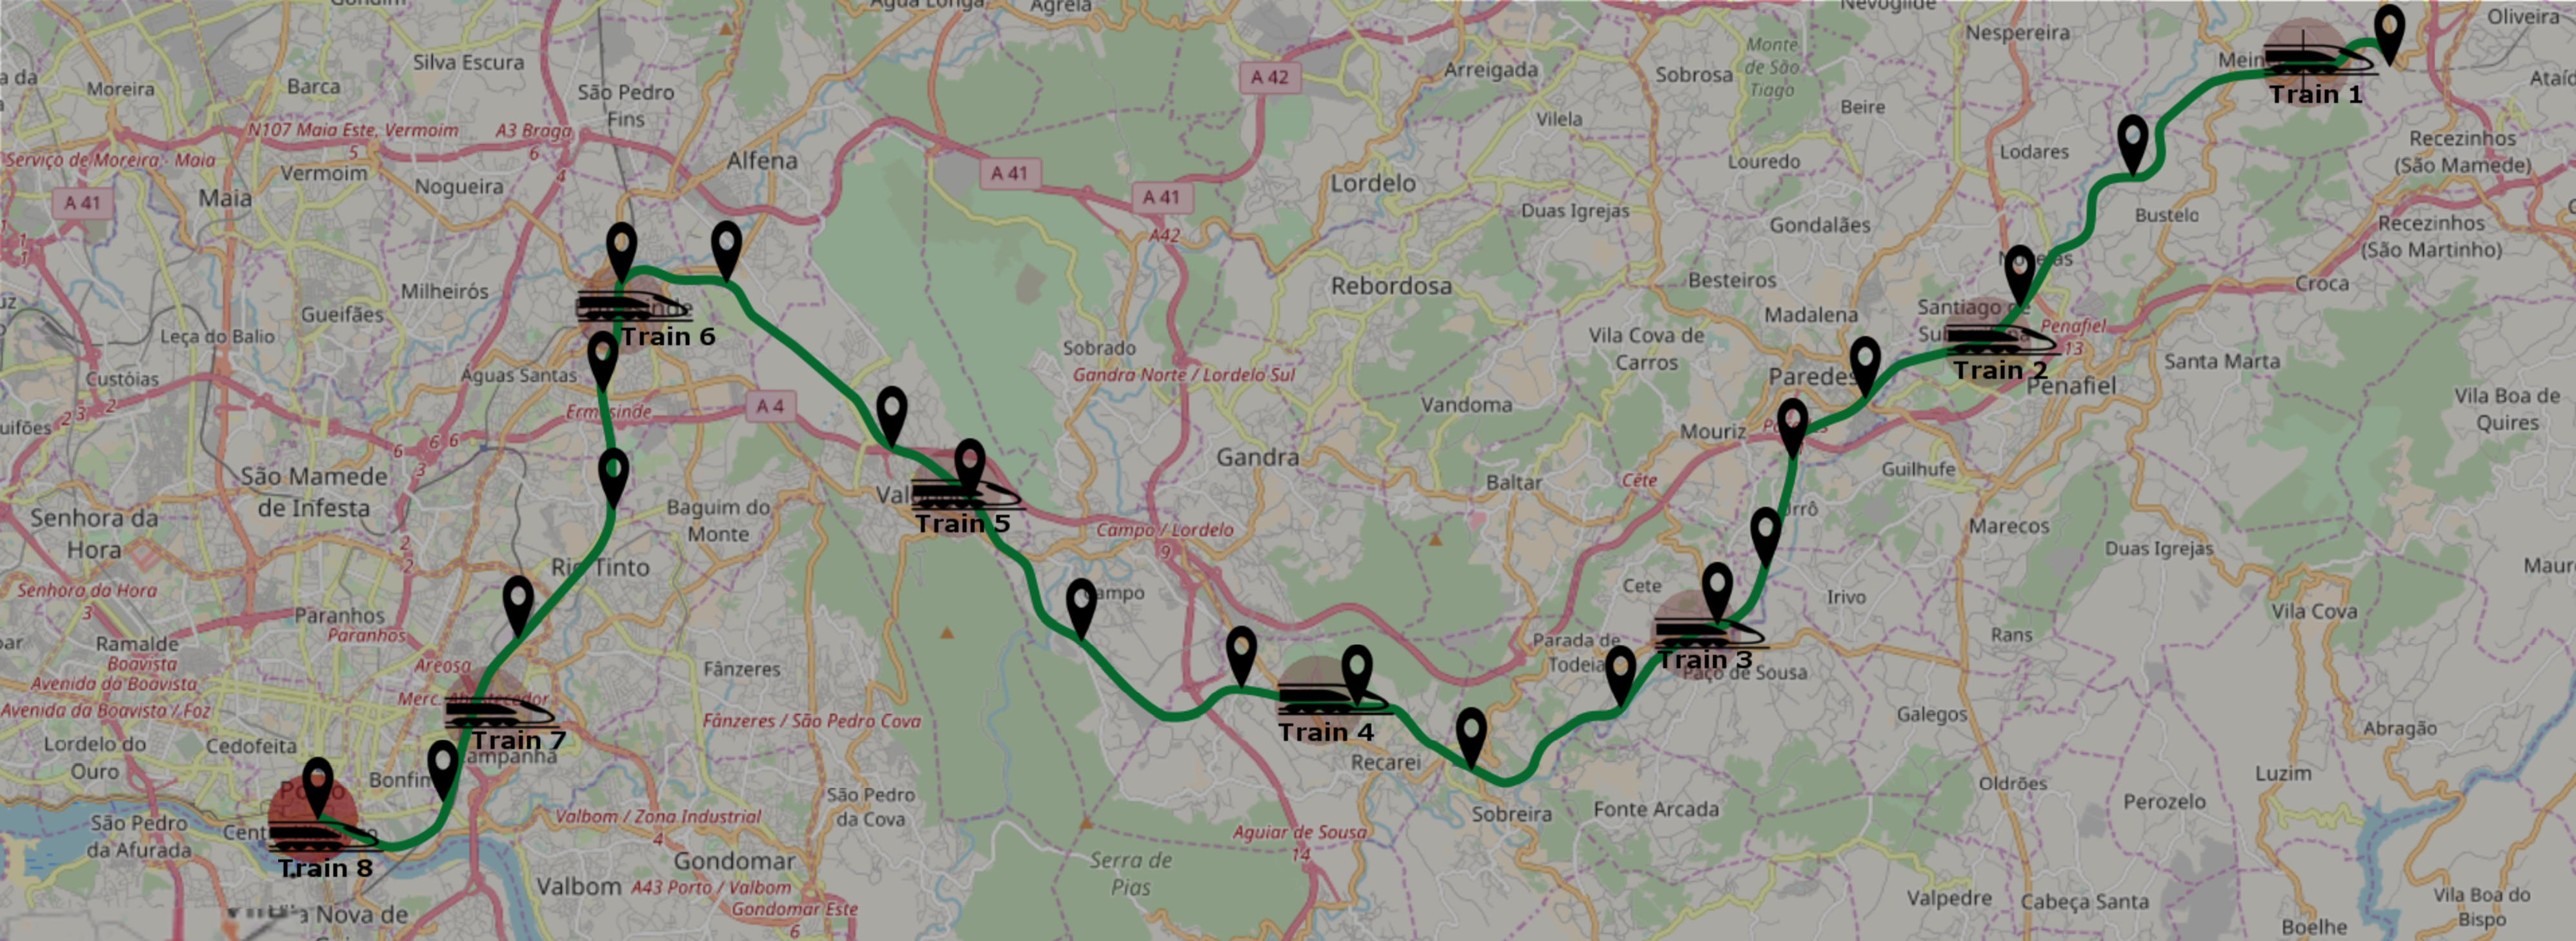
\includegraphics[width=0.9\textwidth,keepaspectratio]{figures/50.PreliminaryW/porto-caide2}
		\caption{Porto-Caíde railway line: simulation using OMNeT++ network simulator.}
	\end{figure}
	
\end{block}
\end{frame}
%%%%%%%%%%%%%%%%%%%%%%%%%%%%%%%%%%%%%%%%%%%%%%%%%%%%%%%%%%%%%%%%%%%%%%%%%%%%%%%%%%%%%

\begin{frame}{Preliminary Work}{Implementation of a point-to-point communication between a moving train and a station}

\begin{figure}[ht!]
	\centering
	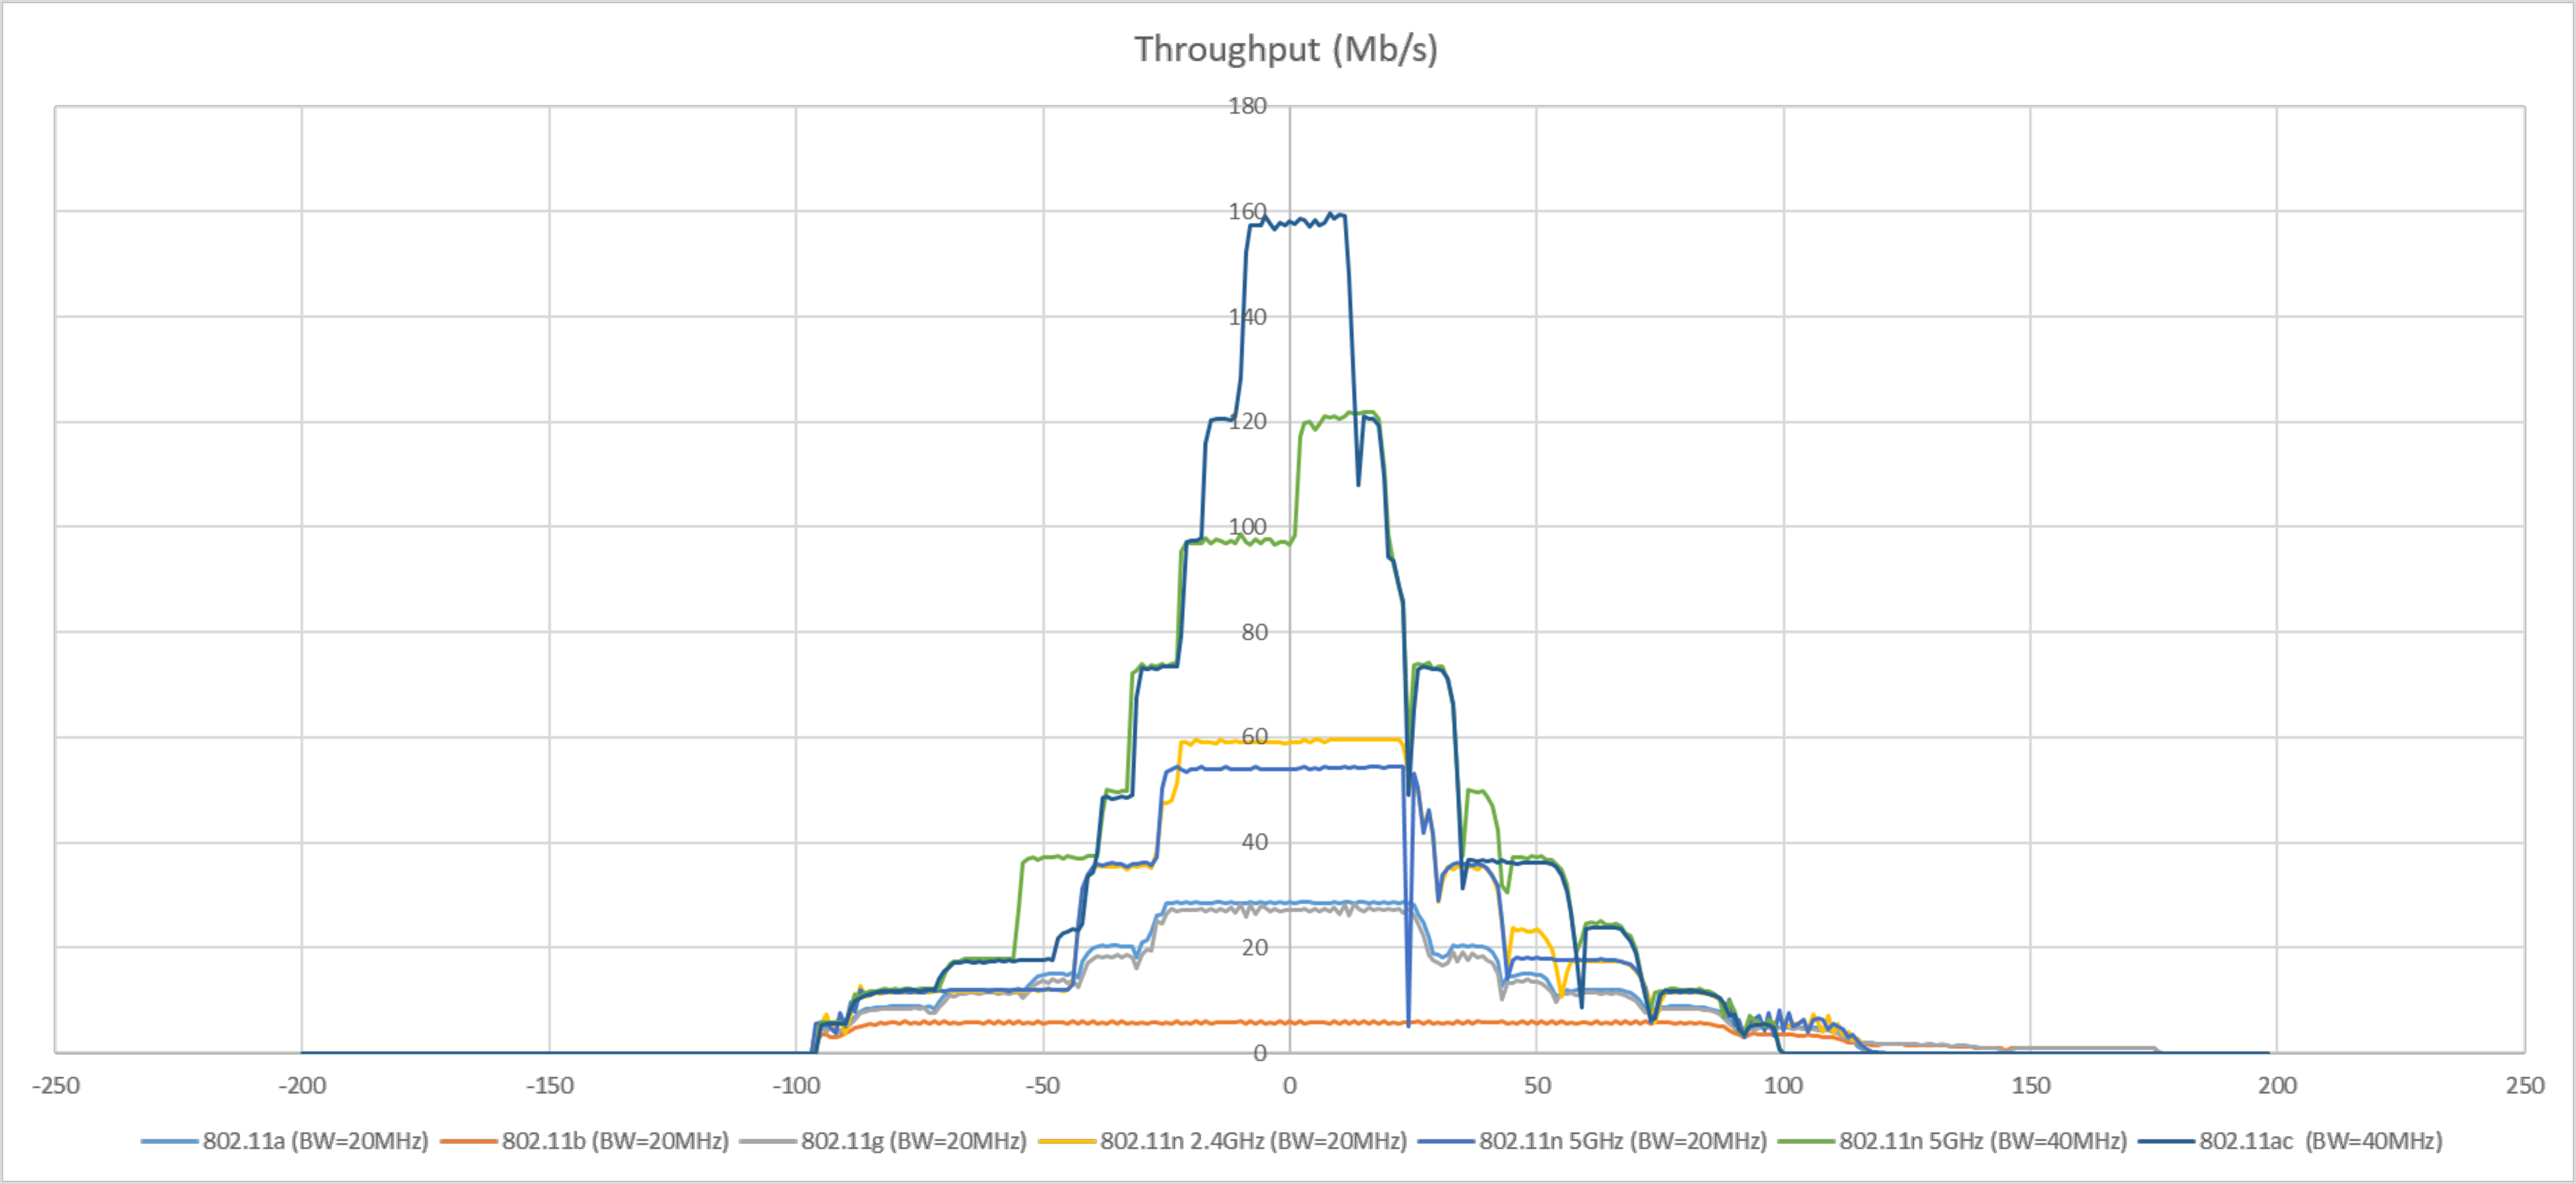
\includegraphics[width=\textwidth,keepaspectratio]{figures/50.PreliminaryW/distance-rate}
	\caption{Evaluation of moving node for different 802.11 network standards using NS-3.}
\end{figure}


\end{frame}
%%%%%%%%%%%%%%%%%%%%%%%%%%%%%%%%%%%%%%%%%%%%%%%%%%%%%%%%%%%%%%%%%%%%%%%%%%%%%%%%%%%%%

\begin{frame}{Preliminary Work}{Implementation of a point-to-point communication between a moving train and a station}

\begin{figure}[ht!]
	\centering
	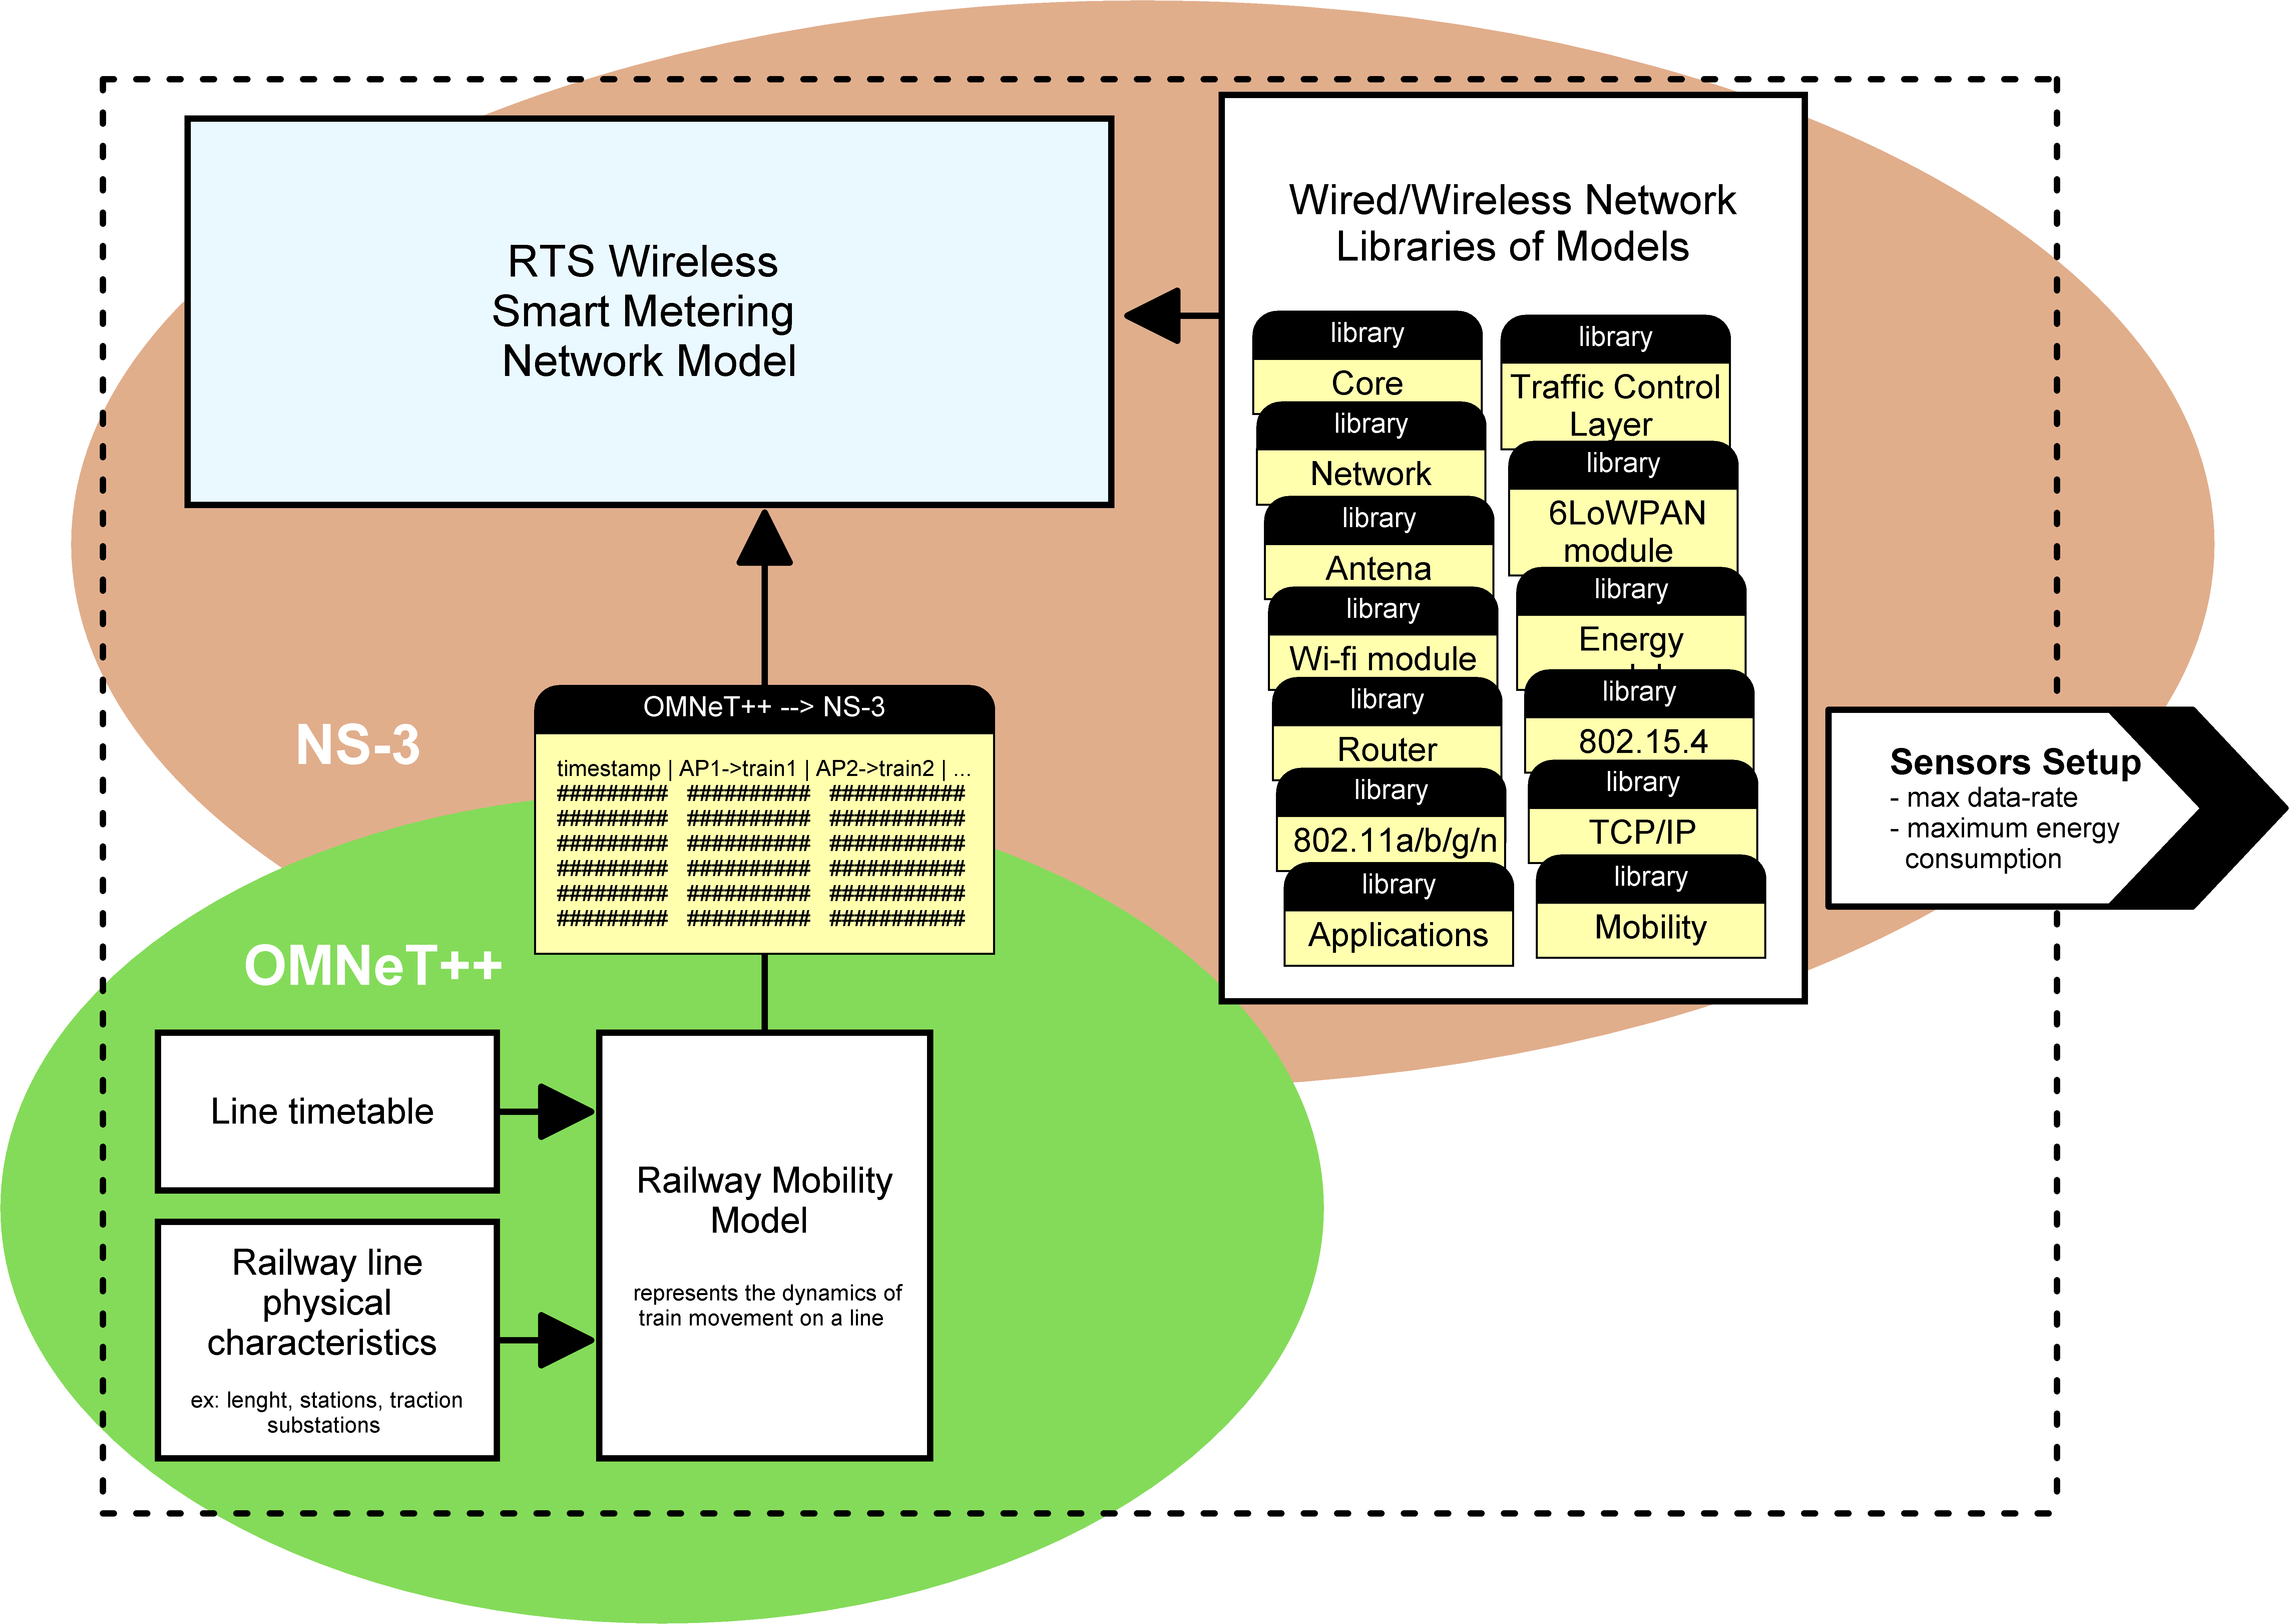
\includegraphics[width=0.70\textwidth,keepaspectratio]{figures/50.PreliminaryW/omnetpp+ns32}
	\caption{Simulator layers: proposed solution using OMNeT++ and NS-3.}
\end{figure}


\end{frame}
%%%%%%%%%%%%%%%%%%%%%%%%%%%%%%%%%%%%%%%%%%%%%%%%%%%%%%%%%%%%%%%%%%%%%%%%%%%%%%%%%%%%%

\subsection{Evaluation of the non-intrusive voltage sensor}

\begin{frame}{Preliminary Work}{Evaluation of the non-intrusive voltage sensor}
\begin{block}{\textbf{Evaluation of the non-intrusive voltage sensor}}
	
		\begin{minipage}[t]{0.51\linewidth}
		
		\begin{figure}[ht!]
			\centering
				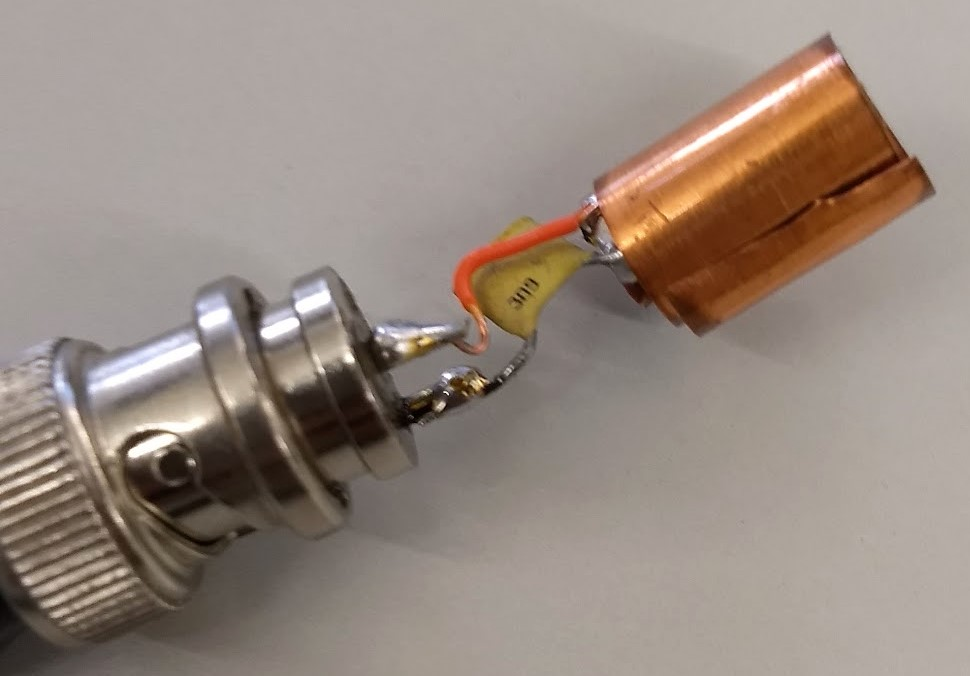
\includegraphics[width=0.43\textwidth,keepaspectratio]{figures/50.PreliminaryW/voltage_sensor}
			%		\vspace{2em}
			\caption{Photo of implemented non-intrusive voltage sensor.}
		\end{figure}
	\end{minipage}\hfill
	\begin{minipage}[t]{0.48\linewidth}
		%\begin{itemize}
		%	\item  50 Hz 25 kV supply system.
		
		%\end{itemize}
		
		\begin{figure}[ht!]
			\centering
			\includegraphics[width=1\textwidth,keepaspectratio]{figures/50.PreliminaryW/generalArchitecture}
			\caption{Signal conditioning and digital processing architecture.}
		\end{figure}
		
		
		
	\end{minipage}
	
	
	
\end{block}
\end{frame}
%%%%%%%%%%%%%%%%%%%%%%%%%%%%%%%%%%%%%%%%%%%%%%%%%%%%%%%%%%%%%%%%%%%%%%%%%%%%%%%%%%%%%

\begin{frame}{Preliminary Work}{Evaluation of the non-intrusive voltage sensor}
\begin{figure}[h!]
	\centering
	\begin{minipage}{.48\textwidth}
		\centering
		%		\vspace{2.5em}
		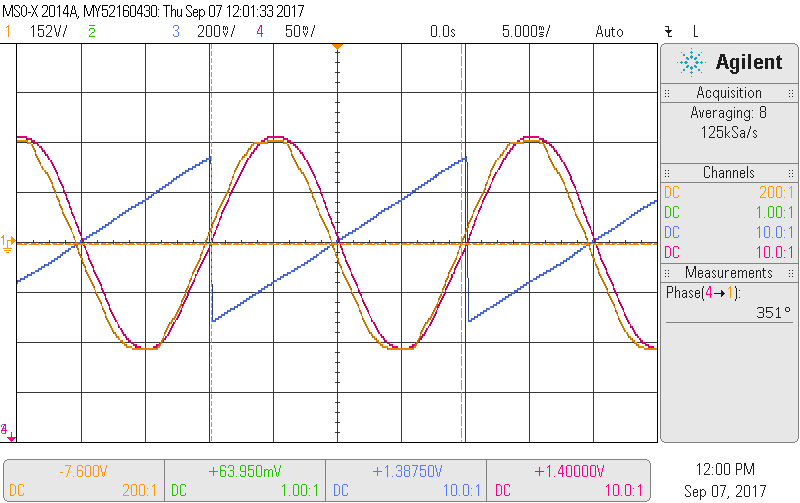
\includegraphics[width=0.95\textwidth,keepaspectratio]{figures/50.PreliminaryW/scope_9}
		%		\vspace{2em}
		\captionof{figure}{Waveforms of AC voltage (orange), estimated voltage (pink) and estimated phase angle (blue) without phase compensation.}
		\label{fig:5.scope_9}
	\end{minipage}%
	\begin{minipage}{.01\textwidth}  ~\end{minipage}	
	\begin{minipage}{.48\textwidth}
		\centering
		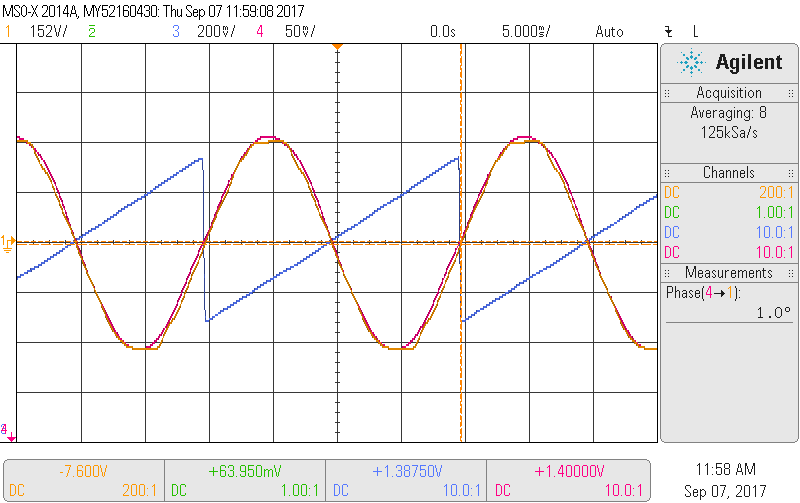
\includegraphics[width=0.95\textwidth,keepaspectratio]{figures/50.PreliminaryW/scope_10}
		%		\vspace{2em}
		\captionof{figure}{Waveforms of AC voltage (orange), estimated voltage (pink) and estimated phase angle (blue) with phase compensation.}
		\label{fig:5.scope_10}
	\end{minipage}
\end{figure}
\end{frame}
%%%%%%%%%%%%%%%%%%%%%%%%%%%%%%%%%%%%%%%%%%%%%%%%%%%%%%%%%%%%%%%%%%%%%%%%%%%%%%%%%%%%%



\begin{frame}
	\subtitle{ }
	\author[]{Thanks for your attention \\ Questions?}
	
	\institute[] % (optional, but mostly needed)
	{
		
	}
	% - Use the \inst command only if there are several affiliations.
	% - Keep it simple, no one is interested in your street address.
	\date{}
	\titlepage
	
\end{frame}

\begin{frame}{Attachments}{Railway Power System Model}

\begin{figure}[ht!]
	\centering
	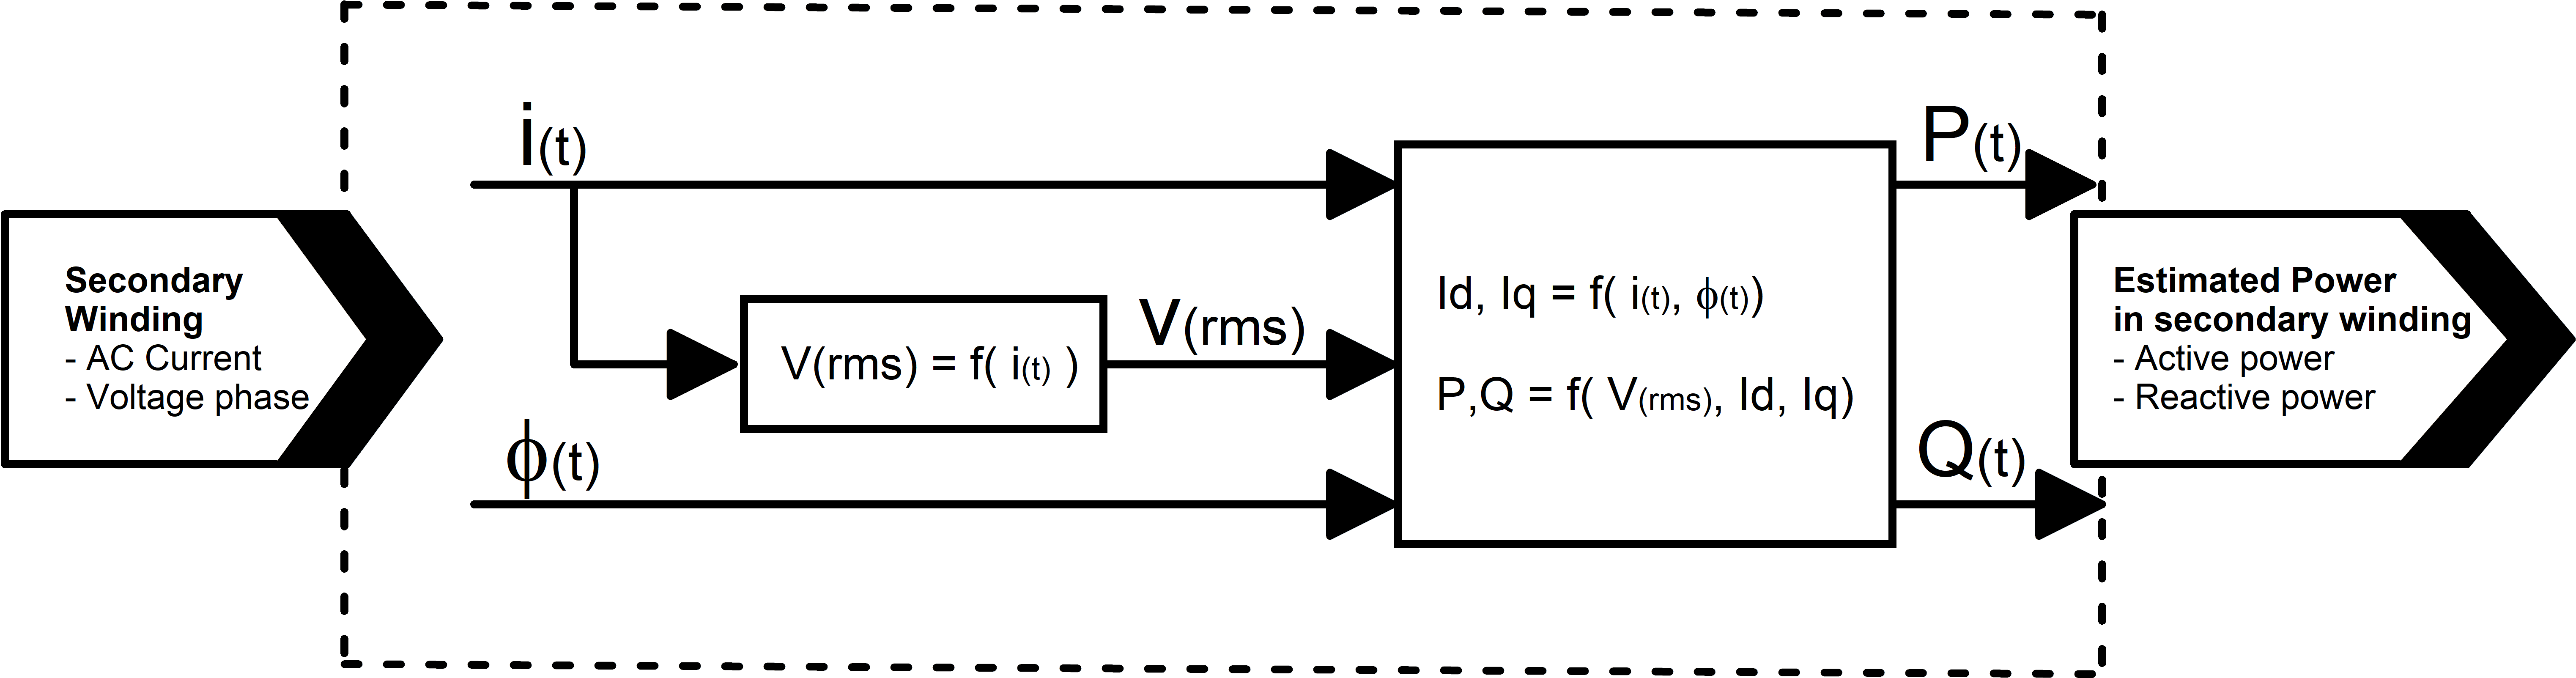
\includegraphics[width=0.8\textwidth,keepaspectratio]{figures/99.aux/voltage_estim}
	\caption{Secondary power estimation.}
\end{figure}

\begin{figure}[ht!]
	\centering
	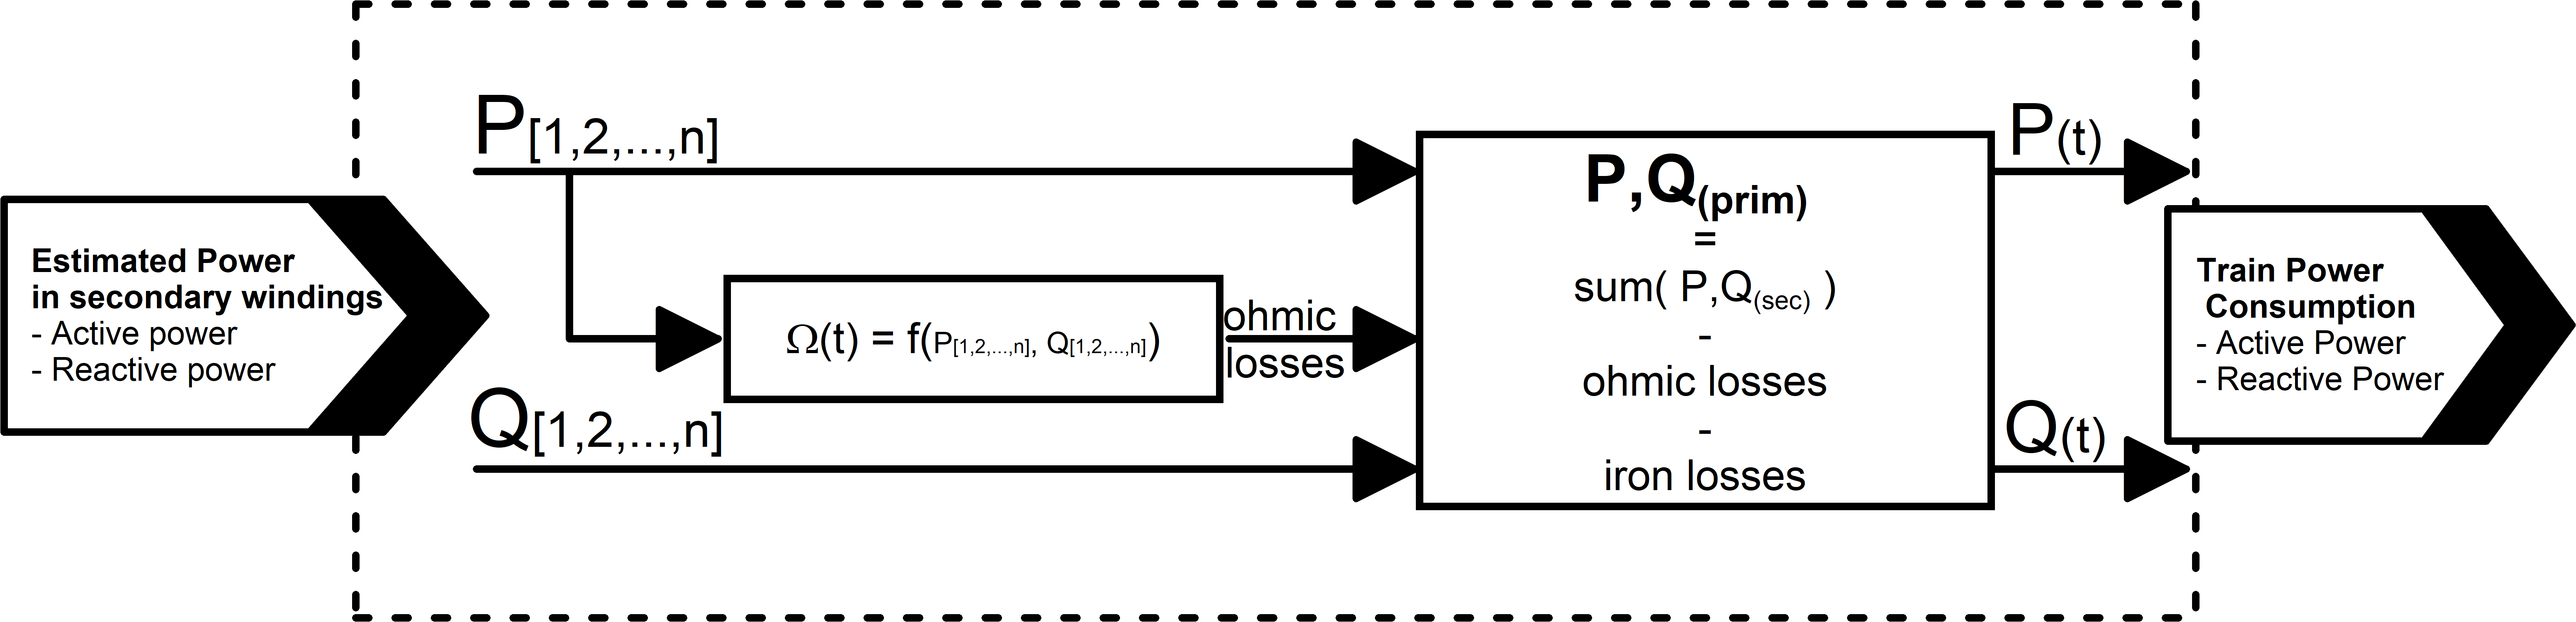
\includegraphics[width=0.8\textwidth,keepaspectratio]{figures/99.aux/train_estim}
	\caption{Train power estimation.}
\end{figure}
\end{frame}
%%%%%%%%%%%%%%%%%%%%%%%%%%

\begin{frame}{Attachments}{Railway Power System Model}
\begin{figure}[ht!]
	\centering
	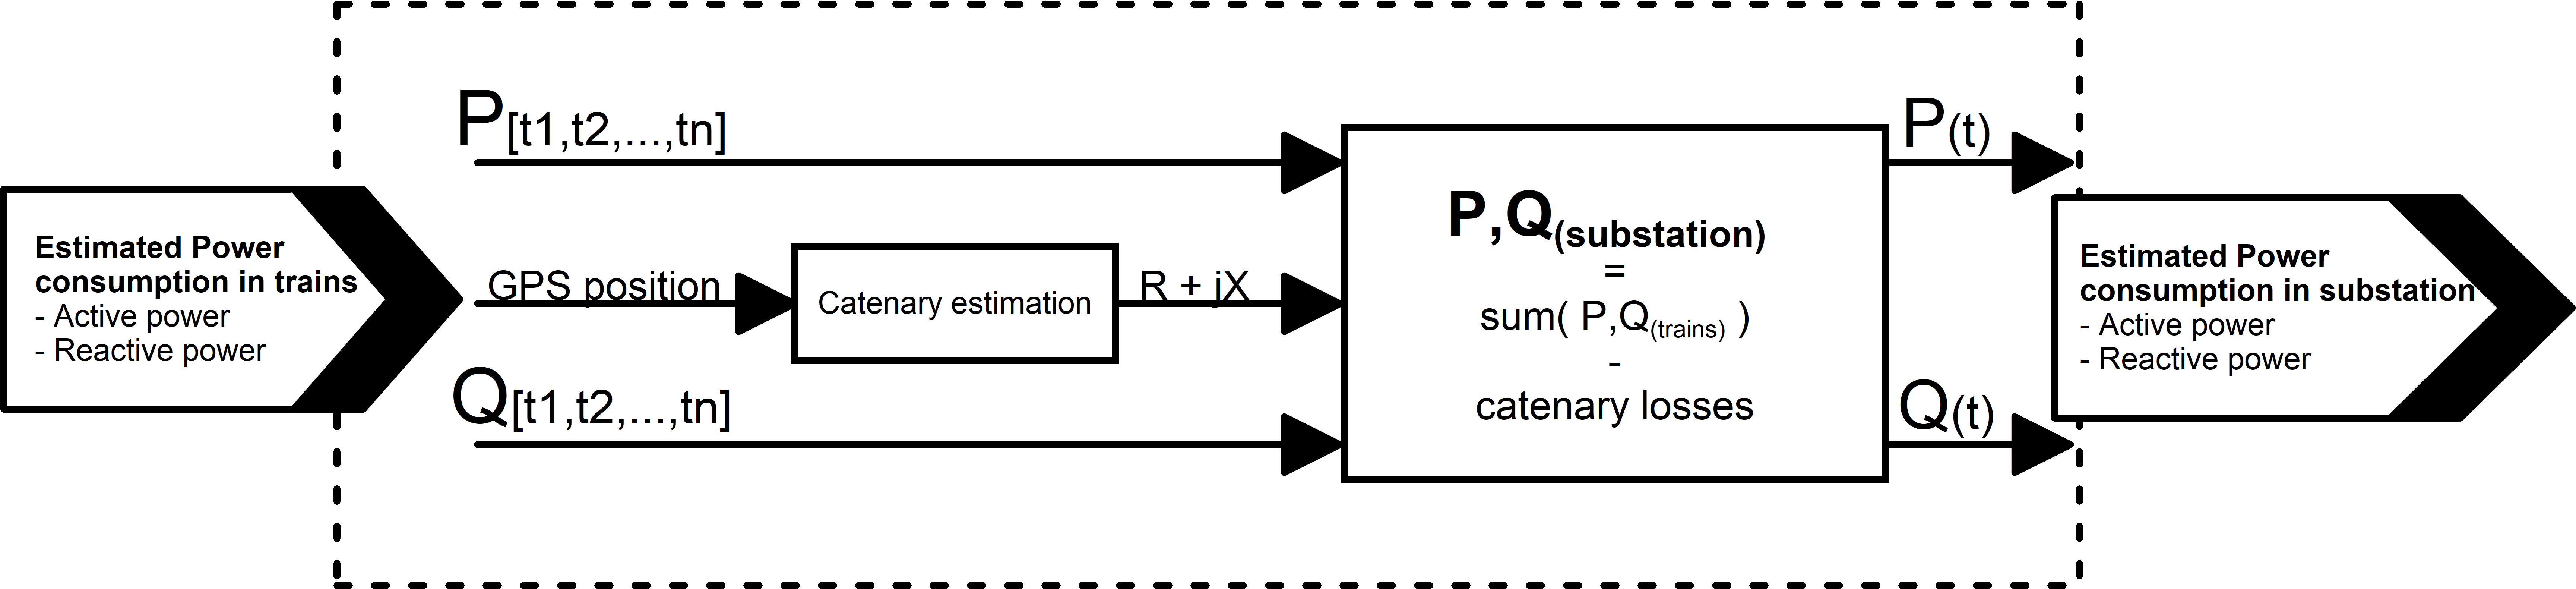
\includegraphics[width=0.9\textwidth,keepaspectratio]{figures/99.aux/substation_estim}
	\caption{Substation power estimation.}
\end{figure}
%\end{block}
\end{frame}


\begin{frame}{Attachments}{Workplan}
\begin{figure}[ht!]
	\centering
	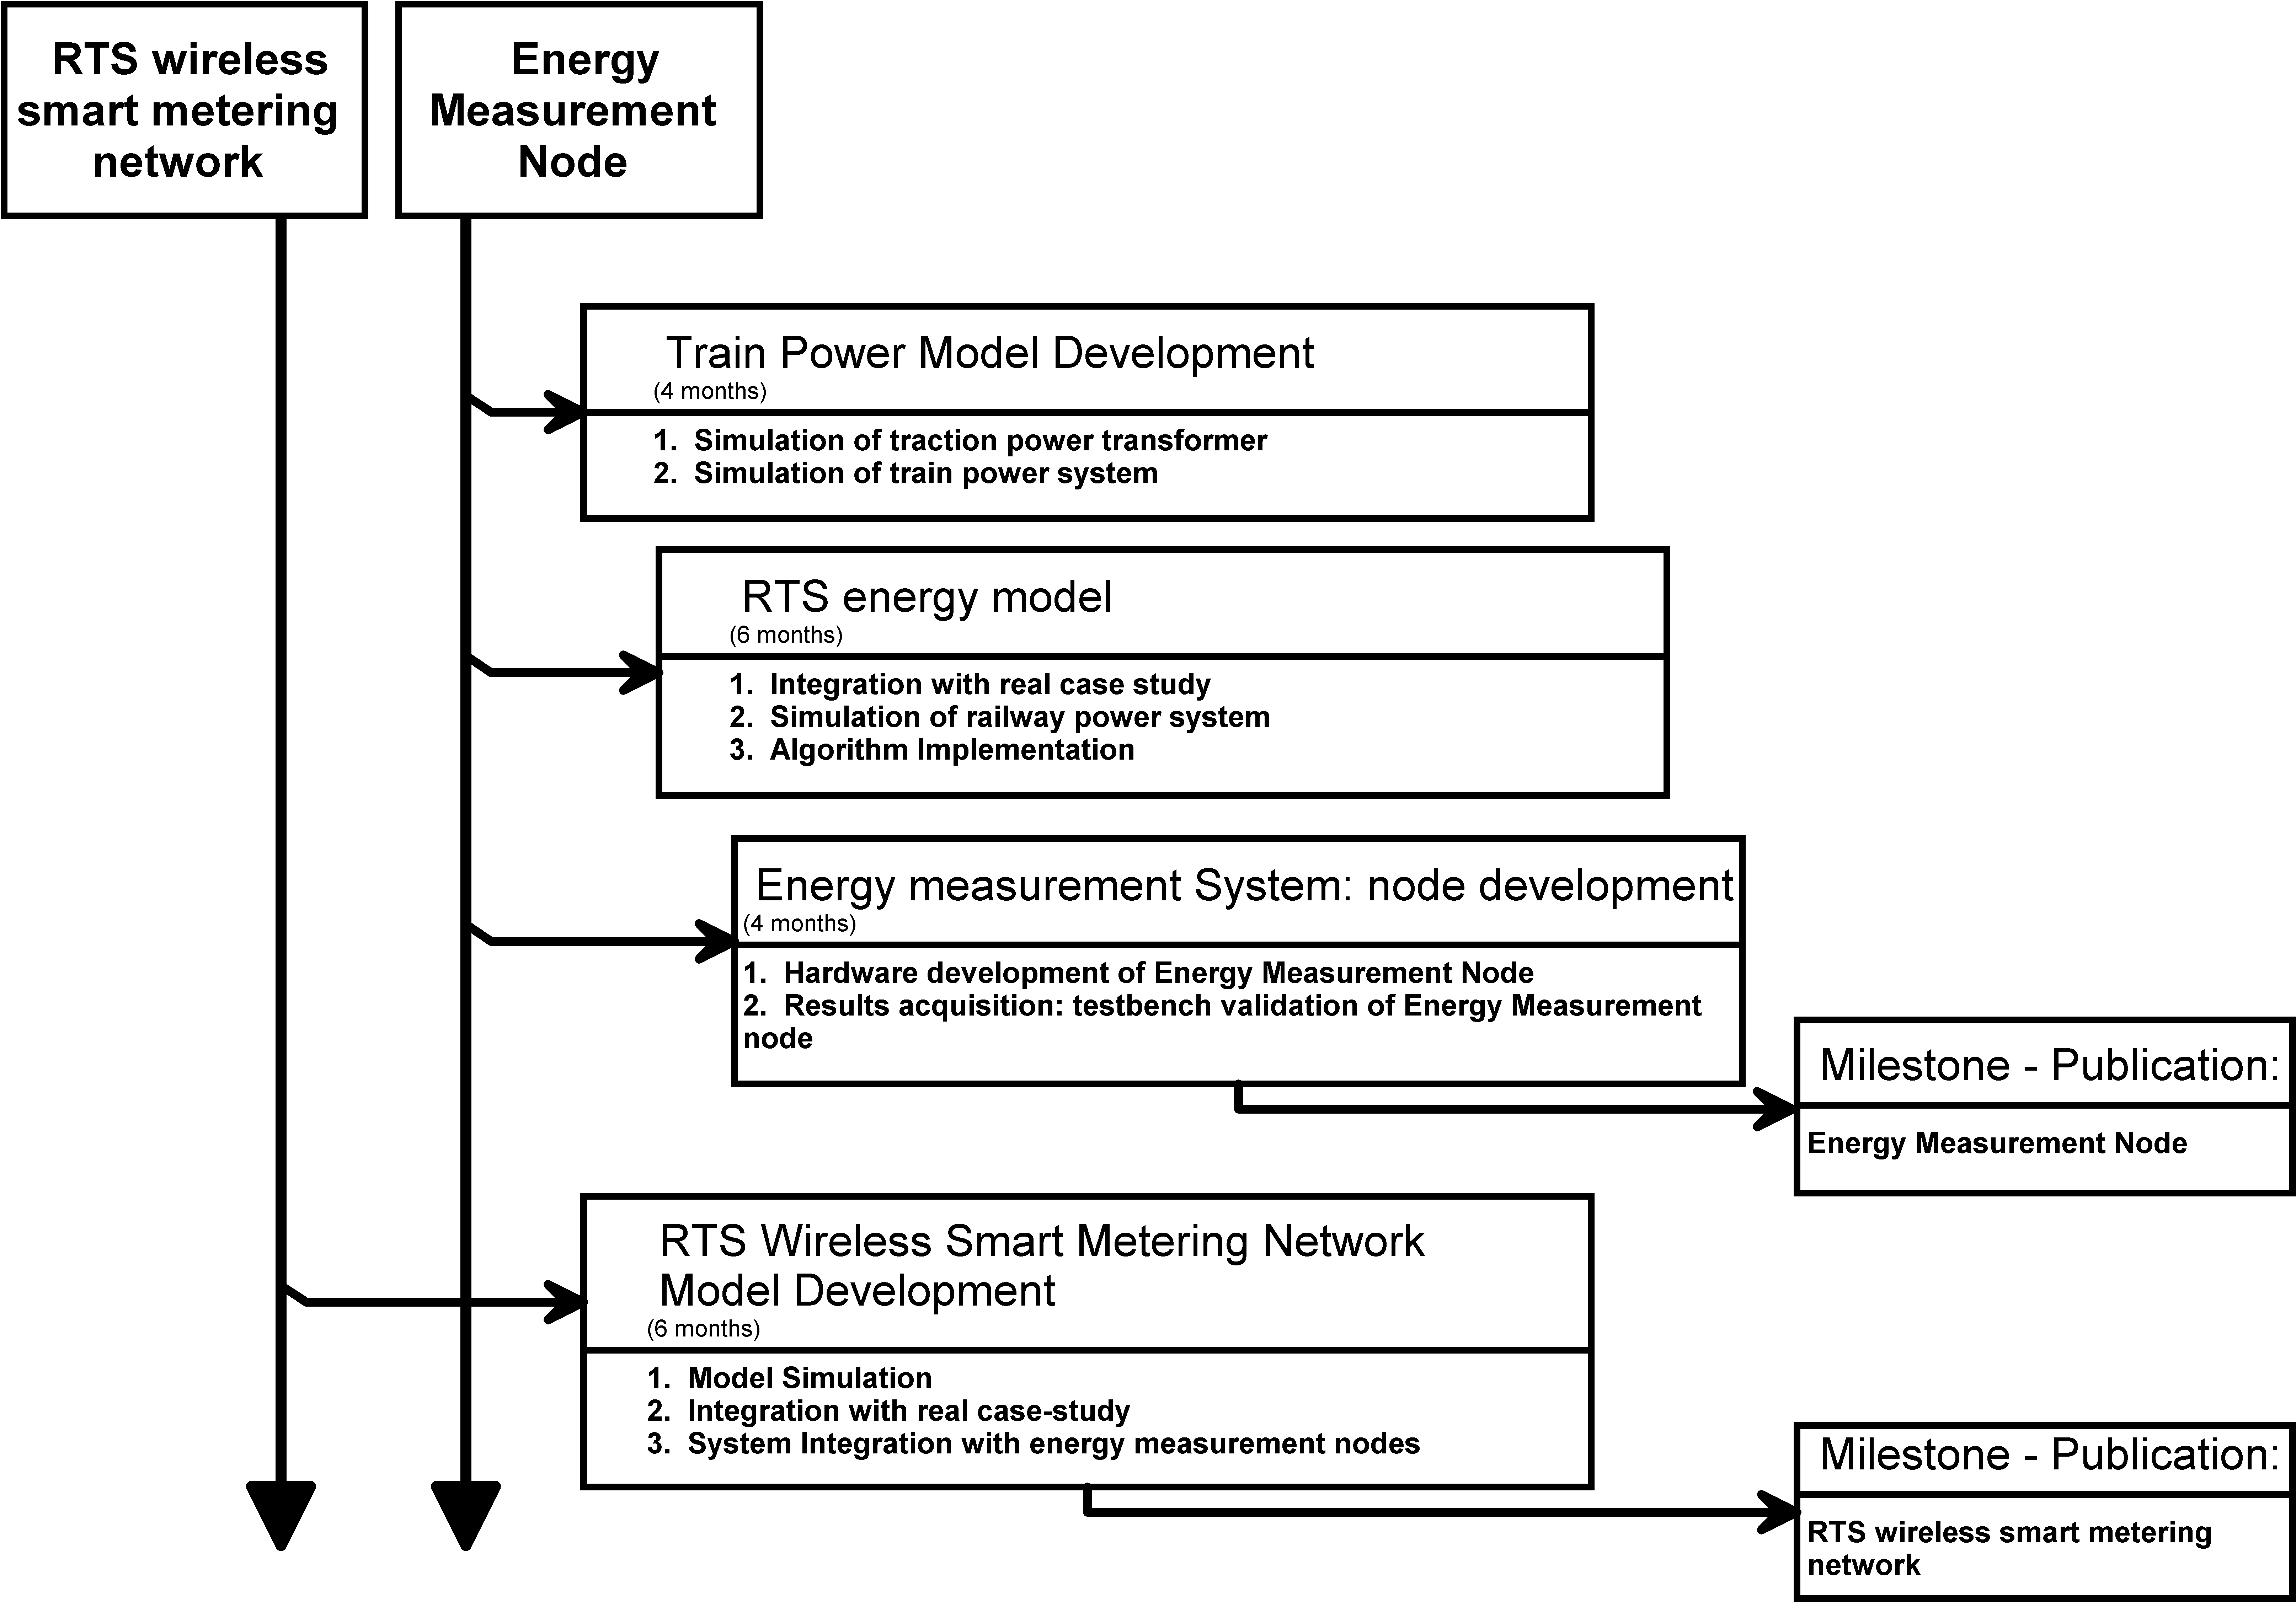
\includegraphics[width=0.8\textwidth,keepaspectratio]{figures/40.Method/workplan1}
	\caption{PhD Work Plan.}
\end{figure}
%\end{block}
\end{frame}

\begin{frame}{Attachments}{Workplan}
\begin{figure}[ht!]
	\centering
	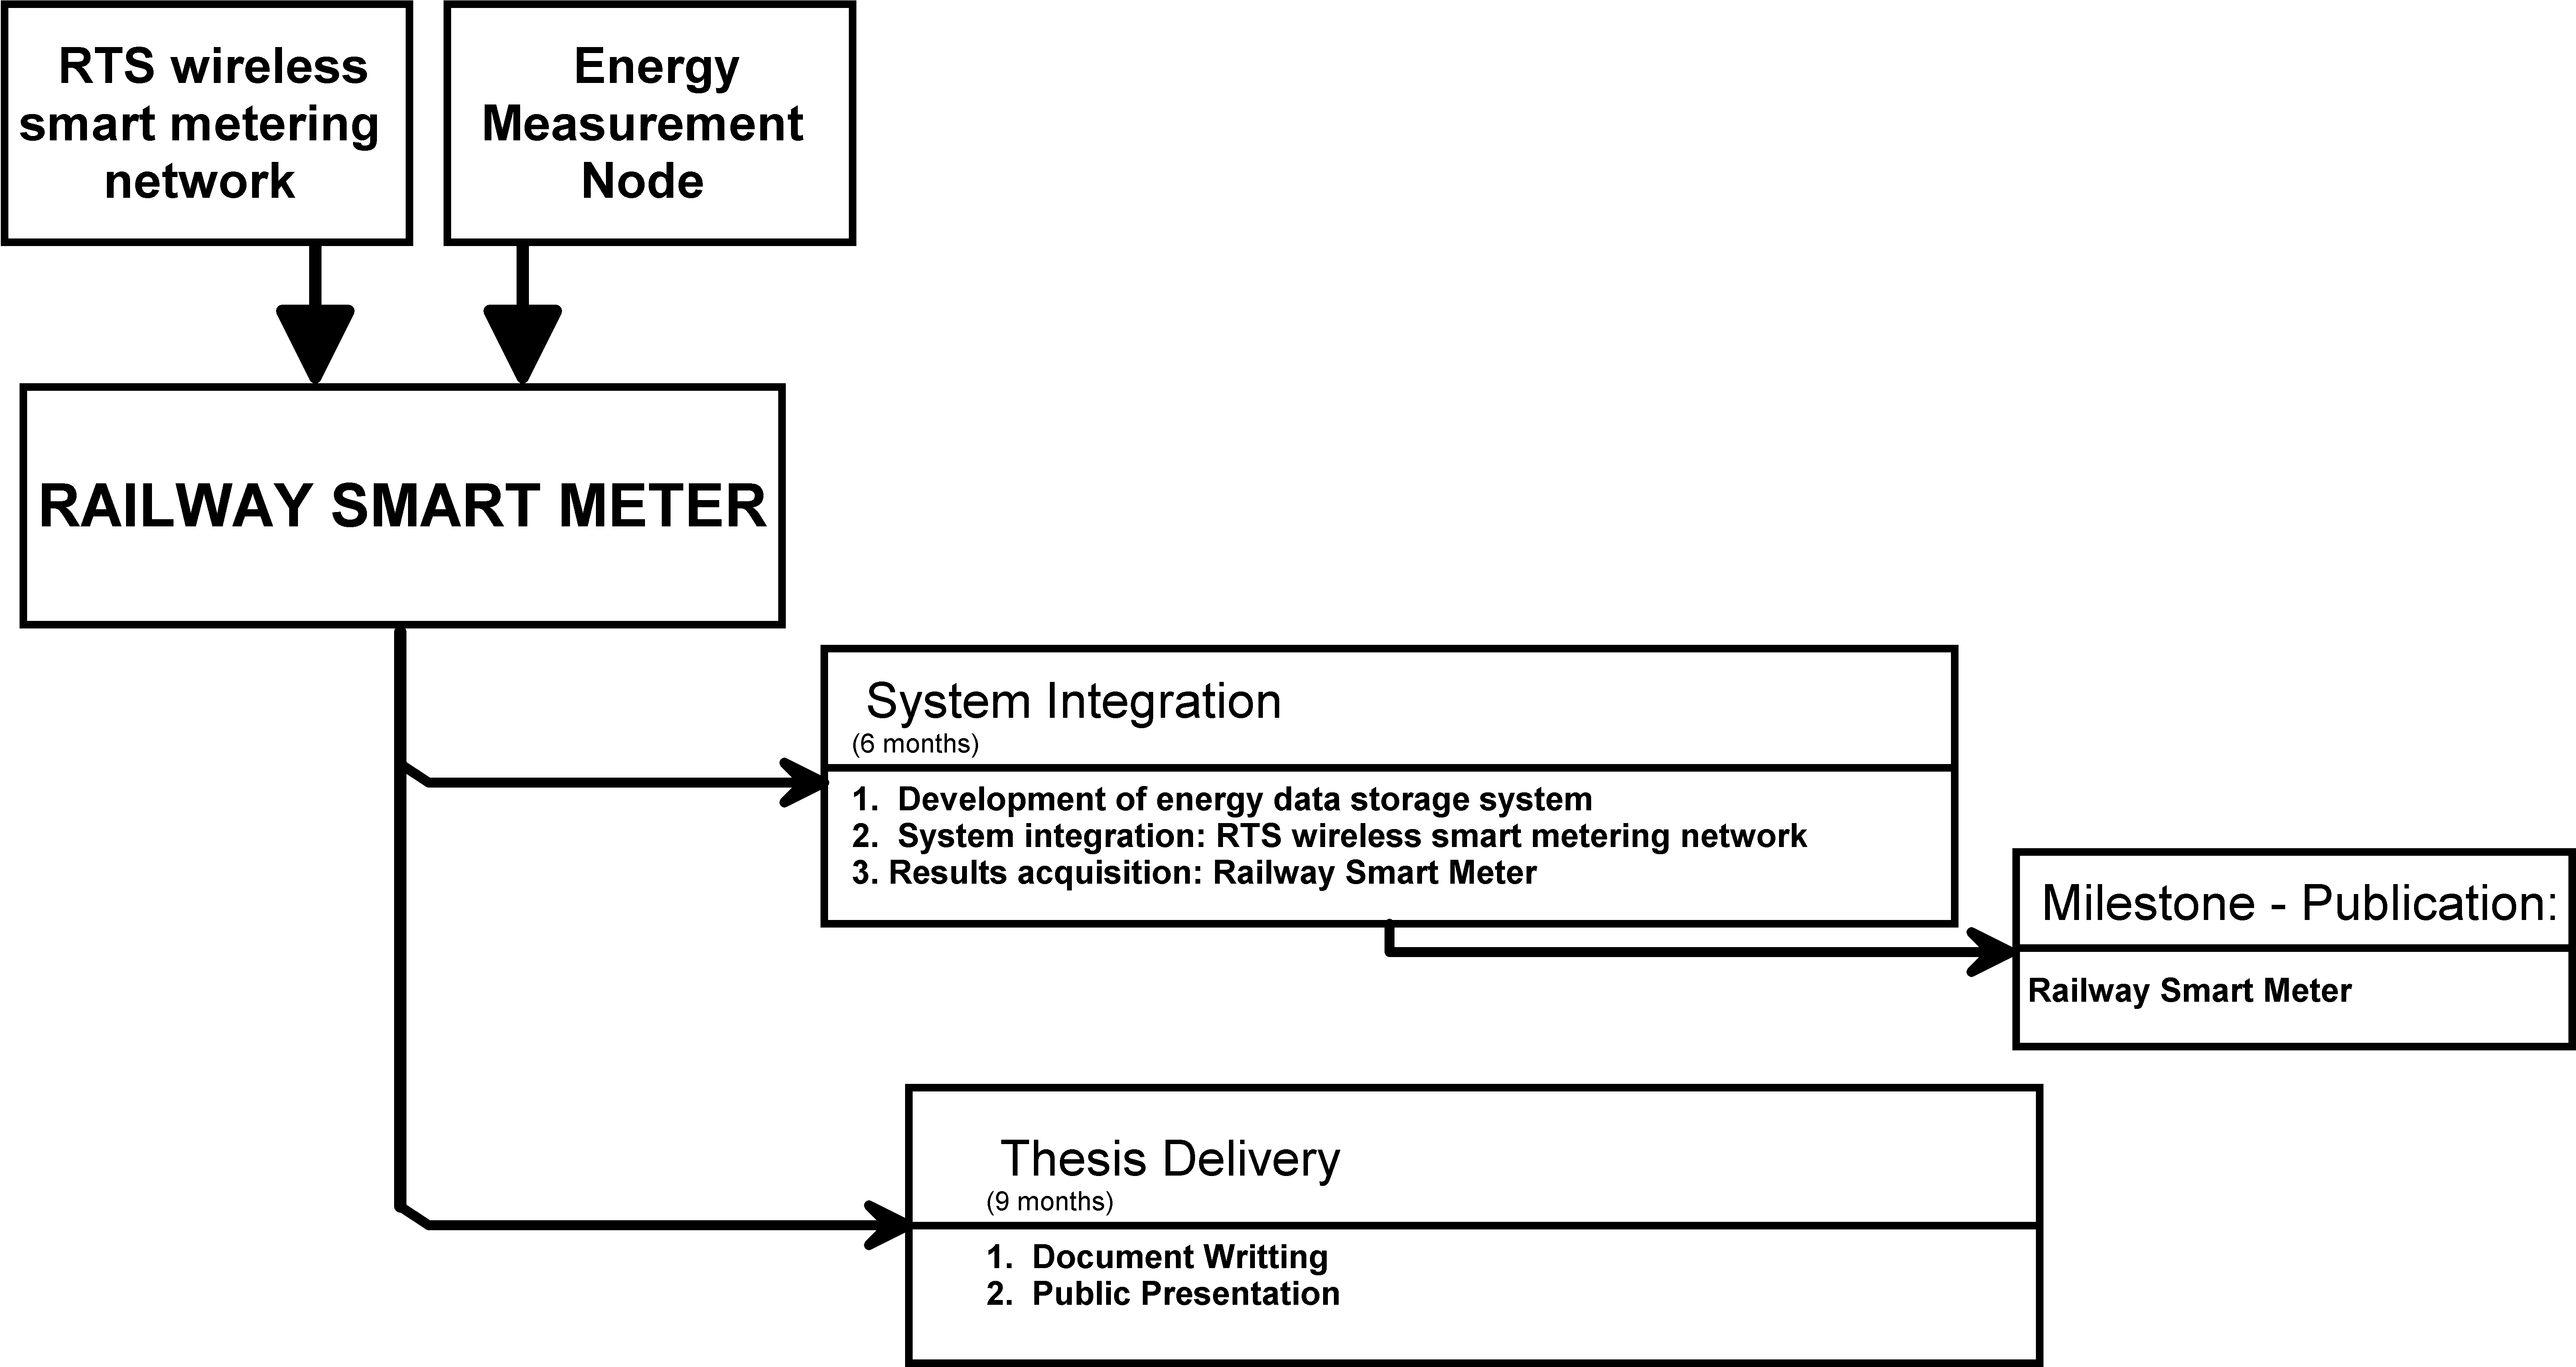
\includegraphics[width=0.8\textwidth,keepaspectratio]{figures/40.Method/workplan2}
	\caption{PhD Work Plan.}
\end{figure}
%\end{block}
\end{frame}


\begin{frame}[allowframebreaks]
	
	\frametitle<presentation>{Bibliography}	
	\bibliographystyle{IEEEtran}
	\bibliography{bib/1.Intro,bib/31.PowerS,bib/32.EnergyS,bib/33.WirelessN,bib/34.SmartM,bib/35.DSS,bib/36.OutlierD,bib/4.Method,bib/5.Preliminary}
	
\end{frame}



\end{document}


